\chapter[Experimental Results and Analysis]{\texorpdfstring{Experimental Results\\and Analysis}{Experimental Results and Analysis}}
\label{chap:experiments}
{%

\section{Experimental Setup}
\label{sec:experimental-setup}

\subsection{Platform and Data}
\label{ssec:platform-and-data}

All experiments are conducted using the CGRSP simulator with per-stratum mean execution times derived from 6,234 real rendering jobs logged by the author's RunPod rendering pipeline between July 2025 and June 2026 (6,030 from its production Serverless endpoint, 203 tagged as development runs and one with no environment tag). Job timestamps are recorded in UTC by the originating AWS Lambda handler (verified against live CloudWatch logs) and are converted to Taiwan time (UTC+8) throughout this thesis for readability. The jobs span four GPU types (RTX~3090: 970 jobs, RTX~A5000: 4,680 jobs, RTX~A4000: 249 jobs, RTX~A4500: 335 jobs), three scene complexity levels, and a wide range of output resolutions (from small preview renders of a few thousand pixels to 48-megapixel stills). In the raw dataset, execution times range from 30 seconds to 352 seconds, with an aggregate coefficient of variation of $\approx$0.27 across the whole dataset and a smaller within-stratum dispersion (pooled $\sigma_{\ln} \approx 0.11$) once complexity and GPU type are fixed. Because the production logs record no scene metadata (polygon counts, materials), the complexity level of each job in the calibration dataset was assigned by render-time terciles of the empirical distribution; the simulator then treats $\kappa_j$ as an observable job attribute, corresponding to a deployment in which the studio classifies complexity from scene statistics known before rendering.

The realised execution time of job $j$ on GPU type $g$ is modelled as a log-normal random variable conditioned on the job's complexity level $\kappa_j \in \{1,2,3\}$ and the GPU type $g$:
\begin{equation}
W(j,g) \sim \text{LogNormal}\!\left(\mu_{\kappa_j,g},\, \sigma_{\kappa_j,g}^2\right),
\qquad
\mu_{\kappa,g} = \ln \overline{W}(\kappa,g) - \tfrac{1}{2}\sigma_{\kappa,g}^2,
\label{eq:lognormal}
\end{equation}
where $\overline{W}(\kappa,g)$ is the empirical mean execution time of the $(\kappa,g)$ stratum in the 6{,}234-job dataset (Table~\ref{tab:gpu_specs}; for a stratum with fewer than five observations it is an estimated mean, flagged in the table where the cell is shown). The location parameter $\mu_{\kappa,g}$ is centred so that $\mathbb{E}[W(j,g)] = \overline{W}(\kappa,g)$; consequently the mean execution times reported throughout this thesis and used in the numerical example (Section~\ref{sec:numerical-example}) are the expected values $\mathbb{E}[W(\kappa,g)]$. The log-normal form is appropriate because render times are strictly positive and right-skewed. The fit is moment-matched rather than tested with a formal goodness-of-fit statistic; the distributional robustness check used here is the mean-based rerun reported later in this section. The dispersion $\sigma_{\kappa,g}$ is fitted per stratum as the standard deviation of $\ln(\text{render time})$ within that stratum, ranging from $0.03$ for the most regular medium-complexity strata to $0.23$ for the most variable high-complexity stratum, with an n-weighted average of the per-stratum values of $\sigma_{\ln} \approx 0.11$ (a within-stratum coefficient of variation of about $0.11$; the variance-pooled standard deviation of the same strata would be about $0.13$); strata with fewer than five observations use that n-weighted average. (The larger aggregate coefficient of variation of $\approx 0.27$ measured across the whole dataset is dominated by between-complexity differences in the mean and is therefore not the relevant conditional dispersion.) The service time $W$ covers the render phase only (the \texttt{render\_time\_s} field of the dataset); the scene-import phase that preceded each render in production (mean 10.8\,s per job, about one seventh of the mean render time) is excluded from both slot occupancy and cost, so simulated per-job occupancy and cost are optimistic by roughly that proportion. The share varies by GPU type, from about 9\% of mean render time on the RTX~A4000 to about 16\% on the RTX~3090, so the size of the bias differs between schedulers that favour different GPU types; adding import time does not change the speed ordering of the four types. Schedulers plan with the deterministic estimate $\overline{W}(\kappa_j,g)$, that is, the expected service time $e_j$; only the realised completion time is stochastic, mirroring real operation where the dispatcher cannot observe a job's exact walltime in advance. Because render walltimes (tens to a few hundred seconds) are small relative to deadline windows ($T_{\text{tight}}$ to $T_{\text{loose}}$) and to queueing delays under saturation, this service-time stochasticity moves mean waits only modestly but matters more for miss rates: in a rerun of the 30 hectic seeds with the log-normal draw replaced by its stratum mean (\texttt{CGRSP/phase3\_diagnostics.py}), mean waits changed by at most \MeanSvcWaitMaxPct\% and miss rates by at most about \MeanSvcMissMaxRelPct\% in relative terms, both for the Adaptive hybrid; no other policy's miss rate moved by more than about 3\%. RH (\MeanSvcRHMiss\% miss) and CADR (\MeanSvcCADRMiss\%) keep their baseline order (paired $p=\MeanSvcRHvCADRp$), so the policy ranking does not hinge on the service noise, although the absolute miss levels in this chapter remain conditional on the log-normal service model. The effect can be slightly larger in lightly loaded, few-seed sub-experiments (for example, the surge-day deadline-tightness sweep), where outcomes near a crossover are more sensitive to the realised service times.

Operational costs are based on RunPod Secure Cloud prices from the 11~March 2026 pricing-API snapshot (Table~\ref{tab:gpu_specs}), treated as fixed deterministic constants throughout all simulations (RunPod prices change over time; these values represent a point-in-time snapshot): RTX~A5000 \$0.27/hr, RTX~3090 \$0.46/hr, RTX~A4500 \$0.25/hr, RTX~A4000 \$0.25/hr. At these Pods snapshot prices, the RTX~3090 is the most expensive GPU in the fleet at \$0.46/hr, approximately 70\% more expensive than the A5000, yet is no faster on the pooled average (72.9\,s vs 72.6\,s for A5000) and has the lower stratum mean only at low and high complexity; this price premium for almost no speed is the primary driver of the cost-aware scheduler designs (RH, CADR, Balanced). The A4500 and A4000 share the same hourly rate (\$0.25/hr) at this snapshot date, so cost differentiation between those two types is absent; the scheduler can exploit the speed difference between them without any cost penalty.

Figure~\ref{fig:data-overview} summarises the empirical dataset. The arrival pattern (panel~a) shows a pronounced peak between 14:00 and 17:00 Taiwan time, consistent with afternoon rendering bursts; the surge-day arrival rate (72 jobs/h) lies below the busiest recorded 60-minute window (119 jobs), whereas the hectic rate (360 jobs/h) is a stress-load assumption about 3.0 times that window. The execution-time distributions (panel~b) confirm right-skewed, GPU-dependent walltimes with medians ranging from 68\,s (RTX~A5000) to 87\,s (RTX~A4000), motivating the per-stratum log-normal service model.

\begin{figure}[H]
\centering
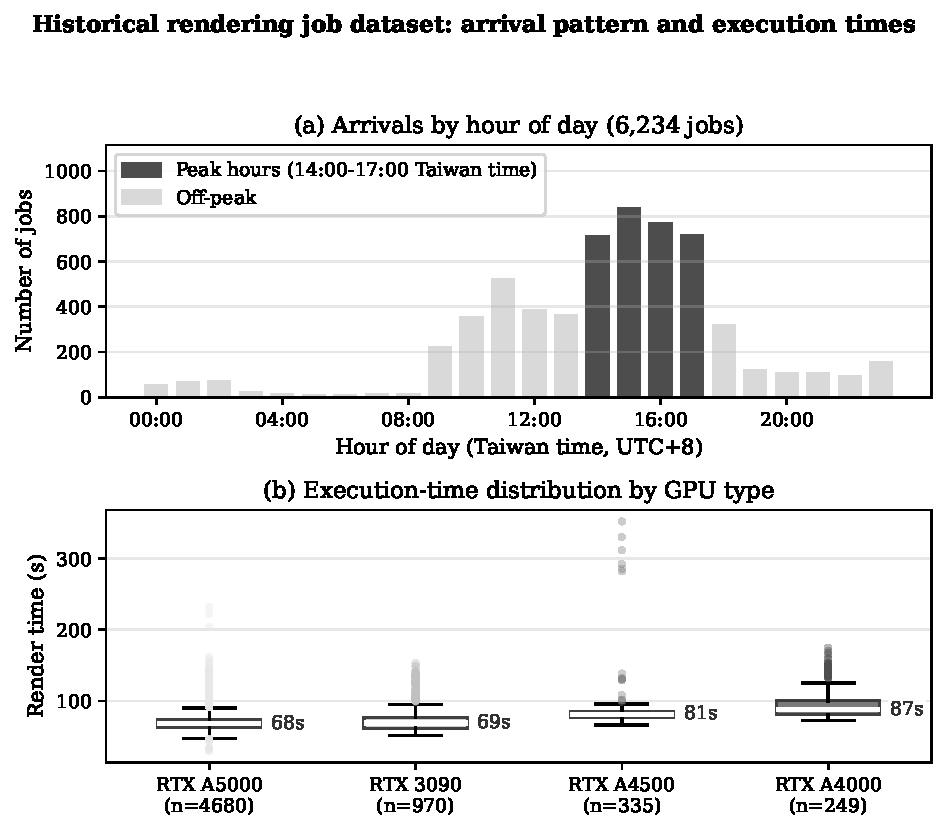
\includegraphics[width=0.97\textwidth]{figures/data_overview.pdf}
\caption[Empirical dataset: arrival pattern and execution times]{Empirical rendering job dataset (6,234 jobs, July 2025 to June 2026). (a)~Hourly arrival counts: the 14:00 to 17:00 Taiwan-time peak (dark grey), which the hectic and surge day types, as stress loads, exceed in daily volume (Section~\ref{ssec:platform-and-data}); off-peak hours are shown in light grey. (b)~Execution-time box plots per GPU type (IQR box, median white line, whiskers at 1.5$\times$IQR, outliers as dots): the RTX~A5000 is fastest (median 68\,s) and the RTX~A4000 slowest (median 87\,s), with right skew in all strata justifying the log-normal service model.}
\label{fig:data-overview}
\end{figure}

The simulation environment parameters are:
\begin{itemize}
  \item Simulation duration: 86,400 seconds (24 hours) per run
  \item Concurrency limit: $C_{\max} = 5$ (a baseline concurrency budget of five simultaneous GPU instances, equal to RunPod's default per-account worker quota~\cite{runpod2026maxworkers}; the quota rises with account balance, so $C_{\max}$ is swept in Table~\ref{tab:cmax_sensitivity})
  \item Job arrival: Poisson process with day-type-calibrated burst rate $\lambda$ and total job count $N_{\text{jobs}}$, a standard queueing-theory assumption representing independent submissions with memoryless inter-arrival times. These are independent parameters: the single-day experiments generate exactly $N_{\text{jobs}}$ candidate jobs with inter-arrival times $\sim\mathrm{Exp}(\lambda)$, so the active arrival window is approximately $N_{\text{jobs}}/\lambda$ seconds; the job count is $N_{\text{jobs}}$, not $\lambda \times 86{,}400$:
  \begin{itemize}[nosep, leftmargin=2em]
    \item Quiet: $\lambda=0.0008$ j/s, 6 jobs/day (arrival window $\approx$2.1\,hr)
    \item Normal: $\lambda=0.002$ j/s, $\sim$100 jobs/day (arrival window $\approx$13.9\,hr)
    \item Hectic: $\lambda=0.100$ j/s, $\sim$950 jobs/day (arrival window $\approx$2.6\,hr; capacity saturation $\rho>1$)
    \item Surge: $\lambda=0.020$ j/s, 730 jobs/day (arrival window $\approx$10.1\,hr)
  \end{itemize}
  The quiet count is of the order observed in the job record. The normal count (100) is above a typical recorded day: the normal-class billing days imply about 27 jobs at RunPod's Serverless Flex rates, and recorded days of 10 to 79 jobs average about 32 (the largest holds 78), so a simulated normal day is moderately loaded rather than typical. The hectic and surge counts are stress-load modelling assumptions rather than counts observed in the job record: the surge count matches the average spend of the surge-class billing days at the same rates (about 750 jobs), but the hectic count is a saturating burst of the order of the single busiest billing day (about 1,070 jobs), roughly ten times what the average hectic-class billing day implies (about 90 jobs); the busiest day in the 6,234-job record holds 415 jobs (18~September 2025, Taiwan time).
  \item Deadline: heterogeneous distribution: 20\% of jobs have a tight 1-hour deadline ($T_{\text{tight}}=3{,}600$\,s, rush orders) and 80\% have a loose 8-hour deadline ($T_{\text{loose}}=28{,}800$\,s, standard renders). Objective weights: $\alpha_1 = 1$ (penalty per second of wait) and $\alpha_2 = 10$ (penalty per missed deadline); the ratio $\alpha_2/\alpha_1 = 10$ is swept in Section~\ref{ssec:objective-weight-sensitivity}. This split is a modelling assumption reflecting a rendering studio context in which a minority of frames are time-critical (client delivery, real-time preview) while the majority are standard batch renders with flexible delivery windows. A uniform deadline distribution would fail to reveal the starvation-deadline trade-off between SPT and SPT+Rescue. The sensitivity of all results to this assumption is assessed explicitly in Section~\ref{ssec:deadline-tightness-sensitivity}, which sweeps the tight-deadline fraction from 10\% to 90\%.
  \item Availability: each rental request incurs a stock-status-dependent provisioning delay $\tau^{\text{prov}}_j$ (formalised in Section~\ref{sec:mathematical-model}, Eq.~\ref{eq:provdelay}). The model treats the platform as an on-demand Secure Cloud pool in which every slot is rentable at any time and a running instance is never reclaimed by the provider, so market scarcity is represented not as denial of service but purely as this provisioning delay. The availability model is informed by RunPod pricing-API snapshots collected between 11~March and 20~April 2026 (5,294 raw snapshots; 77 per-run distribution summaries (usually two runs per collection day) spanning that same 11~March to 20~April collection window were used during calibration): the snapshots supply the secure-cloud hourly prices, the qualitative stock-status vocabulary (High/Medium/Low), and the diurnal demand shape. Snapshot timestamps are tagged UTC by the scraper's own code, but the scraping machine's system clock was in fact running on GMT+7; snapshot hours are therefore shifted by $+1$\,h to Taiwan time (UTC+8) throughout this thesis, consistent with the job-arrival timestamps (which are genuine UTC, shifted by $+8$\,h). The per-type baseline high-stock probabilities $\beta_g$ (RTX~3090 50\%, RTX~A5000 65\%, RTX~A4500 70\%, RTX~A4000 75\%) are \emph{modelling assumptions} for the on-demand secure pool rather than empirical frequencies from the snapshot record: the stock-status field returned by the pricing API (queried for a single-GPU Secure Cloud offer) reports the four fleet types as almost never High and, in a substantial share of snapshots, with no Secure Cloud offer at all (Figure~\ref{fig:availability-history}); read literally this would imply intermittent denial of service, which the model deliberately excludes, so $\beta_g$ encodes an assumed probability that an on-demand request is fulfilled promptly rather than a frequency read from that field. The time-of-day multiplier $\phi(t)$ scales the high-stock probability and is expressed on the simulator's own local clock, which is Taiwan time throughout this project: off-peak, 00:00 to 06:00 ($\times$1.3); morning, 06:00 to 12:00 ($\times$0.9); peak, 12:00 to 18:00 ($\times$0.5); evening, 18:00 to 24:00 ($\times$1.0); the observed record supports this shape qualitatively, with Secure Cloud availability of the fleet types visibly worse during the business-hours peak (Figure~\ref{fig:availability-history}b). Simulation time zero is anchored to 08:00 on the modelled day, matching a studio working day that opens in the morning rather than at midnight, so every run starts in the morning band; the offset is applied arithmetically rather than read from the host machine's clock, so the sequence of bands a run traverses does not depend on the timezone it happens to execute under. Outside the peak band the multiplier keeps $p^{H}_g + p^{M}_g \ge 1$ for all four fleet types, so the Low state is then unreachable; only during the peak band (multiplier $\times 0.5$) does it become reachable at all, and there for all four types, with per-draw probability largest for the low-$\beta_g$ types (37.5\% for the RTX~3090 down to 6.25\% for the RTX~A4000). Because the peak occupies a minority of the day, the time-weighted Low probability is modest, but it is not negligible: instrumenting the delay draw over ten seeds of the FIFO, SPT and EDF runs in the Phase~3 day-type sensitivity runs gives Low-range delays (600\,s or more) on about 3\% of dispatches on hectic and surge days, about 7 to 11\% on normal days (where the few jobs arrive spread across the day, so a larger share meet the peak band), and none on quiet days; on the Phase~4 monthly calendar the shares are about 5 to 8\% on normal days and small but non-zero (about 0.3 to 1.1\%) on quiet days; all other delays are in the High and Medium ranges (at most two minutes). Provisioning delays are drawn uniformly from stock-status ranges: High 0 to 10\,s, Medium 30 to 120\,s, Low 600 to 7200\,s. (Implementation note: the status a scheduler observes is the draw made at the most recent earlier dispatch, and every type reads High before a run's first dispatch. The status realised at acquisition is a fresh, independent draw from the same time-varying model. The observation therefore behaves like a stale marketplace poll rather than a binding quote: apart from what the type's $\beta_g$ and the time-of-day band already imply, it carries no information about the delay the dispatched job then pays. The same observation mechanism applies to every scheduler.) Figure~\ref{fig:diurnal-model} shows the $\phi(t)$ step function alongside the real job arrival pattern; the 77 calibration snapshots are concentrated at hours 02:00 to 03:00 and 19:00 to 20:00 Taiwan time, so $\phi(t)$ is a parametric calibration rather than a pointwise empirical fit.
\end{itemize}

\begin{landscape}
\begin{figure}[H]
\centering
\captionsetup{font=small,skip=6pt}
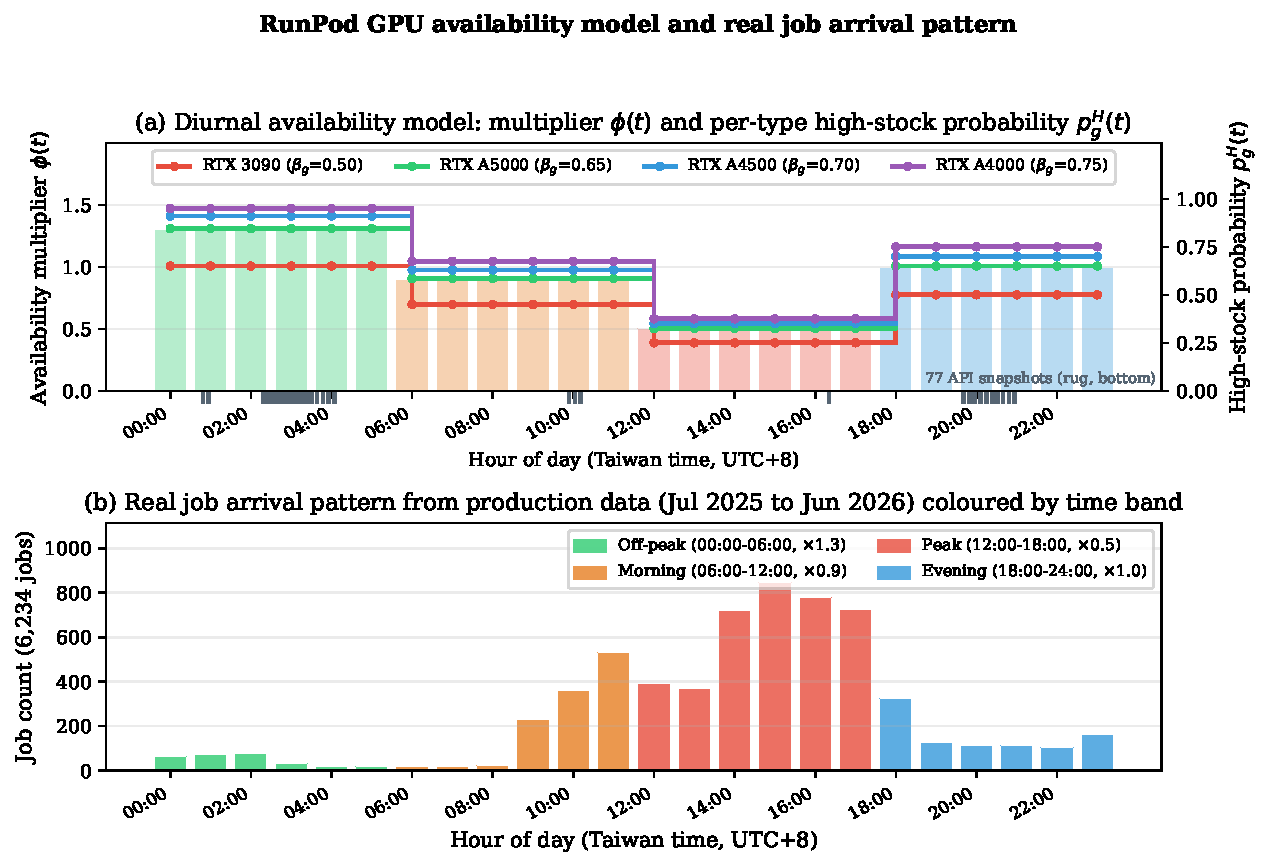
\includegraphics[width=0.98\linewidth,height=0.90\textheight,keepaspectratio]{figures/diurnal_model.pdf}
\caption[Diurnal availability model and real arrival pattern]{Diurnal availability model and real arrival pattern.}
\label{fig:diurnal-model}
\end{figure}
\end{landscape}

\noindent\textit{Figure~\ref{fig:diurnal-model} notes.} Diurnal availability model and real job arrival pattern, all times Taiwan time (UTC+8), matching the simulator's own local clock (Section~\ref{sec:mathematical-model}). (a)~Bars (left axis) show the parametric step function $\phi(t)$: off-peak 00:00 to 06:00 raises availability ($\times$1.3, green); morning 06:00 to 12:00 moderately reduces it ($\times$0.9, orange); peak 12:00 to 18:00 reduces availability by half ($\times$0.5, red); evening 18:00 to 24:00 is neutral ($\times$1.0, blue). Lines (right axis) show the resulting per-type high-stock probability $p_g^H(t) = \min(0.95,\,\beta_g\,\phi(t))$ for each of the four fleet GPUs, using each type's baseline $\beta_g$ (RTX~3090 50\%, RTX~A5000 65\%, RTX~A4500 70\%, RTX~A4000 75\%): the four curves share $\phi(t)$'s step shape but sit at different levels set by $\beta_g$, and the RTX~A4000 curve flattens against the 0.95 ceiling during the off-peak band ($0.75 \times 1.3 = 0.975 \to 0.95$). Rug marks at the bottom show the 77 RunPod API snapshot times, which are concentrated in two narrow windows. (b)~Actual hourly job count from the 6,234 logged rendering jobs (July 2025 to June 2026; 6,030 production, 203 development, one untagged), coloured by the corresponding $\phi(t)$ band. The historical arrival peak at 14:00 to 17:00 Taiwan time falls inside the peak band, so the busiest hours of the production record coincide with the model's lowest-availability window. The simulated day is anchored differently: simulation time zero corresponds to 08:00 Taiwan time (Section~\ref{ssec:platform-and-data}), so a run opens in the morning band ($\times$0.9), and the hectic day's arrival window of roughly 2.6~hours lies wholly inside it; only the longer surge and normal arrival windows extend into the afternoon peak at all. Panel~(b) therefore describes when the studio historically submitted work; in the simulated hectic day the arrivals fall in the morning band, while the saturated backlog they create is still being dispatched through the afternoon peak band, where stock status and provisioning delay are drawn at dispatch time.\par

\begin{landscape}
\begin{figure}[H]
\centering
\captionsetup{font=small,skip=6pt}
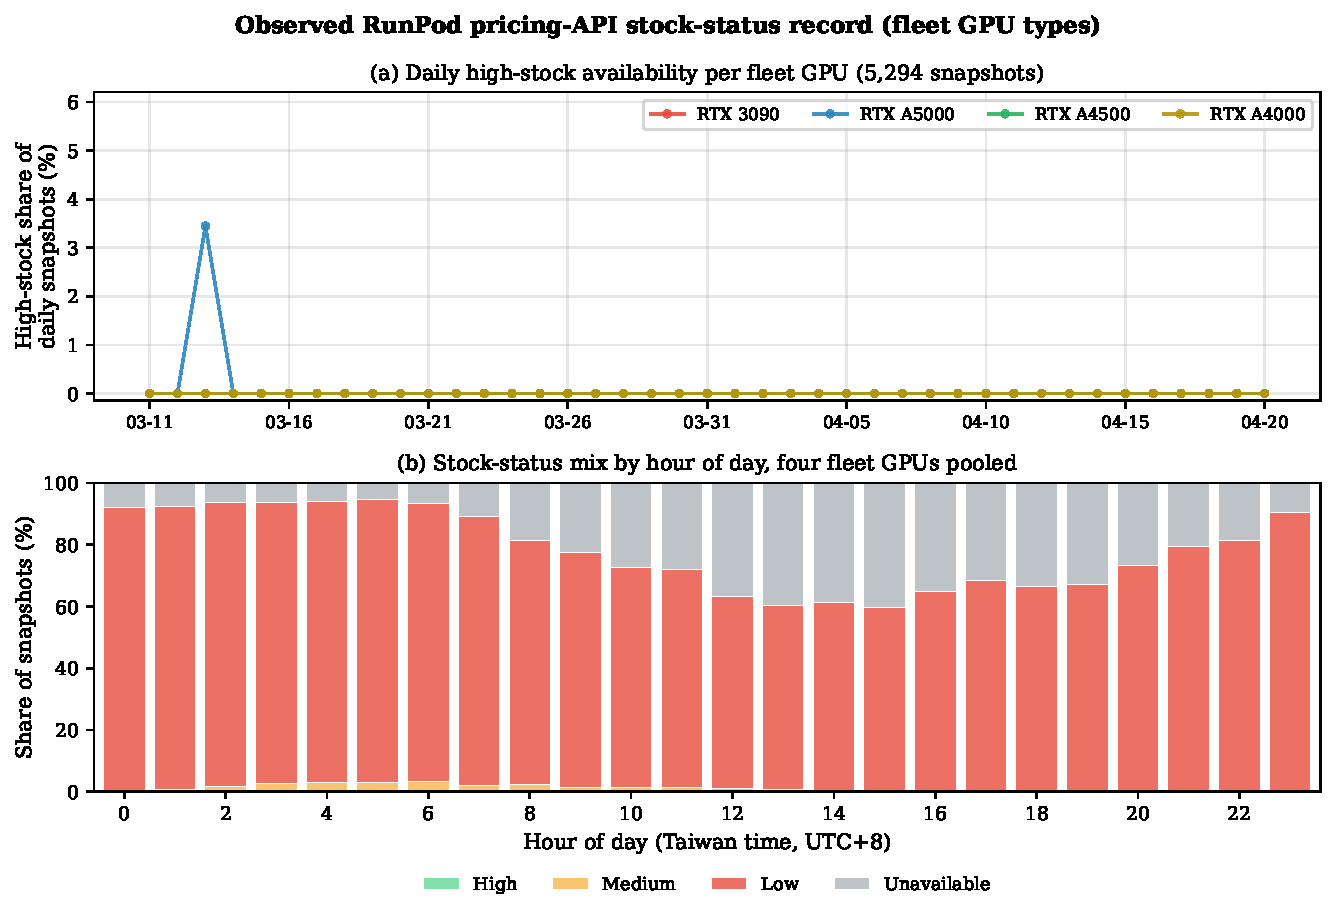
\includegraphics[width=0.98\linewidth,height=0.85\textheight,keepaspectratio]{figures/availability_history.pdf}
\caption[Observed RunPod availability record]{Observed RunPod availability record.}
\label{fig:availability-history}
\end{figure}
\end{landscape}

\noindent\textit{Figure~\ref{fig:availability-history} notes.} Observed RunPod availability record for the four fleet GPU types, 11~March to 20~April 2026 (5,294 pricing-API snapshots). (a)~Daily share of snapshots reporting High stock: essentially zero throughout the collection window. (b)~Stock-status mix by hour of day (fleet types pooled): the Secure Cloud single-GPU listing for these consumer-tier types is chronically Low-stock, and the share of snapshots with no Secure Cloud offer (Unavailable) rises during the business-hours window, qualitatively consistent with the peak-demand reduction encoded in $\phi(t)$. Because the model excludes the no-offer state this record shows, the baseline high-stock probabilities $\beta_g$ are treated as modelling assumptions for the on-demand pool; the snapshot record contributes the fleet prices, the stock-status vocabulary, and the diurnal demand shape.\par

\subsection{Evaluation Phases}
\label{ssec:evaluation-phases}

Four phases of evaluation are conducted (phases are numbered from 2; Phase~1 comprised initial exploratory calibration runs not reported here):

\begin{description}
  \item[Phase 2] Single-seed benchmark (seed=42) on the hectic-day configuration of Section~\ref{ssec:platform-and-data}. Provides illustrative point estimates for the seven baseline schedulers (all but RH, CADR and the Adaptive hybrid) under capacity saturation ($\rho>1$; RH, CADR, and the Adaptive hybrid enter at Phase~3); being single-seed it carries no confidence interval and is superseded by the $n=30$ Phase~3 statistics for every inferential claim.
  \item[Phase 3 Statistical] 30 independent replications (seeds 0 to 29) on hectic-day workload ($\sim$950 jobs/day). Computes 95\% confidence intervals and paired $t$-tests (with a Wilcoxon signed-rank backup) and Cohen's $d$ for pairwise comparisons. Includes RH, CADR, and the CADR-order-only (CADR-OO) ablation variant. Tardiness (mean minutes past deadline) is reported as a diagnostic alongside miss rate.
  \item[Phase 3 Sensitivity] Compares all schedulers across four operationally calibrated day types (quiet/normal/hectic/surge) at $C_{\max}=5$, with 30 seeds per day type (1{,}200 total runs). Identifies the load regime where scheduler differences become operationally significant.
  \item[Phase 4] 30-day monthly simulation (10~replications; the type of each day, one of quiet, normal, hectic and surge, is drawn from day-of-week probabilities estimated by classifying the 30 complete days of RunPod billing between 22~April and 21~May 2026 by daily spend). Aggregates scheduler performance across monthly workload variation to assess behaviour over a mixed month. Each replication uses one persistent fleet and queue for all 30 days. Daily Poisson traces are capped at the sampled candidate job count and cut off at the next day boundary; jobs already accepted continue across boundaries, and after the final boundary the simulator drains the remaining backlog. Metrics are grouped by submission day and use accepted jobs as the denominator. Ten replications rather than 30 were used because each replication simulates a complete calendar; 10 replications yield 95\% CIs with $t^*_9 = 2.262$, providing adequate precision for the monthly comparison objective.
\end{description}

A \textbf{deadline tightness sensitivity} study sweeps tight-deadline fraction $f_{\text{tight}} \in \{10\%,\allowbreak 30\%,\allowbreak 50\%,\allowbreak 70\%,\allowbreak 90\%\}$ under surge-day conditions ($C_{\max}=5$, $\lambda=0.020$ j/s, 730 jobs/day, 30 seeds each) to identify the load regime where EDF's deadline-safety advantage over SPT is maximised.

\subsection{Statistical Methodology}
\label{ssec:statistical-methodology}

All statistical comparisons use a paired $t$-test on the per-seed averages, with a Wilcoxon signed-rank test~\cite{wilcoxon1945individual} as a distribution-free backup. Every scheduler is evaluated on the same 30 seeds with identical generated jobs per seed, so the per-seed observations are matched (a randomised block design); the paired test is therefore both valid and more powerful than an unpaired alternative, as it removes the between-seed variance that the schedulers share. Effect sizes are reported as Cohen's $d = (\mu_1 - \mu_2) / s_{\text{pooled}}$, where $s_{\text{pooled}}$ is the pooled standard deviation. The threshold $|d| \geq 0.8$ is used as the criterion for a practically meaningful effect (``large'' by Cohen's convention~\cite{cohen1988statistical}). Confidence intervals are computed as $\bar{x} \pm t^*_{n-1} \cdot (s/\sqrt{n})$ with $t^*_{29} = 2.045$ for $n=30$, $\alpha=0.05$. For each pairwise comparison it prints, Table~\ref{tab:ttests} also reports the paired mean difference with its 95\% confidence interval, $\bar{d} \pm t^*_{29}\, s_d/\sqrt{n}$, so that each printed effect is stated with its uncertainty~\cite{kalibera2020quantifying,krishnamachari2026statistical}. The $t$-based intervals and tests rely on the per-seed means being approximately normally distributed, which the central limit theorem supports for averages over independent replications~\cite{law2000simulation}; because the number of replications this requires depends on how skewed the underlying metric is, the Wilcoxon signed-rank test above serves as the distribution-free check. Consistent with the lexicographic objective (Eq.~\ref{eq:objective}), which prioritises QoS over operational cost rather than collapsing them into one scalar, all experimental comparisons report each component separately (average waiting time, deadline miss rate, operational cost) rather than as an aggregate. Decomposed reporting enables direct identification of which dimension drives scheduler differences: a scheduler that reduces miss rate by increasing waiting time would appear identically weighted in a scalar objective but the trade-off is transparent in the decomposed view. Each pairwise comparison in Table~\ref{tab:ttests} tests a pre-specified directional hypothesis grounded in scheduling theory (e.g.\ SPT reduces wait by shortest-job-first ordering; EDF reduces miss by deadline ordering) rather than a data-driven hypothesis selection; a Holm-Bonferroni step-down correction~\cite{holm1979simple} over the full pairwise family is nonetheless applied to control the family-wise error rate; as reported below, most but not all comparisons significant at the uncorrected level survive it.

\section{Phase 2: Seven-Scheduler Benchmark}
\label{sec:phase-2-seven-scheduler-benchmark}

Table~\ref{tab:phase2} and Figure~\ref{fig:phase2} report Phase~2 results for all seven schedulers on a hectic day; Figure~\ref{fig:phase2} additionally contrasts a normal day (top row), where all schedulers achieve near-zero miss, to show that the saturated hectic day is the regime in which scheduler choice matters.

\begin{table}[htbp]
\centering
\caption[Phase 2 benchmark results]{Phase 2 benchmark: hectic day ($\sim$950 jobs/day), $C_{\max}=5$, seed=42, $\lambda=0.100$ j/s, 20\% tight 1h / 80\% loose 8h deadlines (capacity saturation: $\rho>1$). Util is event-sampled (mean of per-event fleet-occupancy samples over the active window), not a time-weighted day average.}
\label{tab:phase2}
\begin{tabular}{lrrrrr}
\toprule
\textbf{Scheduler} & \textbf{Avg Wait (min)} & \textbf{Miss \%} & \textbf{Cost (\$)} & \textbf{Util (\%)} & \textbf{Completed} \\
\midrule
\textbf{SPT+Rescue} & 144.02 & \textbf{9.37} & 6.28 & 95.7 & 950/950\\
\textbf{SPT} & \textbf{140.02} & 19.16 & 6.25 & 95.7 & 950/950\\
EDF & 174.21 & 12.11 & 6.30 & 95.7 & 950/950\\
LCF & 157.06 & 16.95 & 6.24 & 95.7 & 950/950\\
Balanced & 174.09 & 24.53 & 6.33 & 95.7 & 950/950\\
FIFO & 165.26 & 23.37 & 6.40 & 95.7 & 950/950\\
Random & 174.35 & 25.26 & 6.34 & 95.7 & 950/950\\
\bottomrule
\end{tabular}

\end{table}

\begin{landscape}
\begin{figure}[H]
\centering
\captionsetup{font=small,skip=6pt}
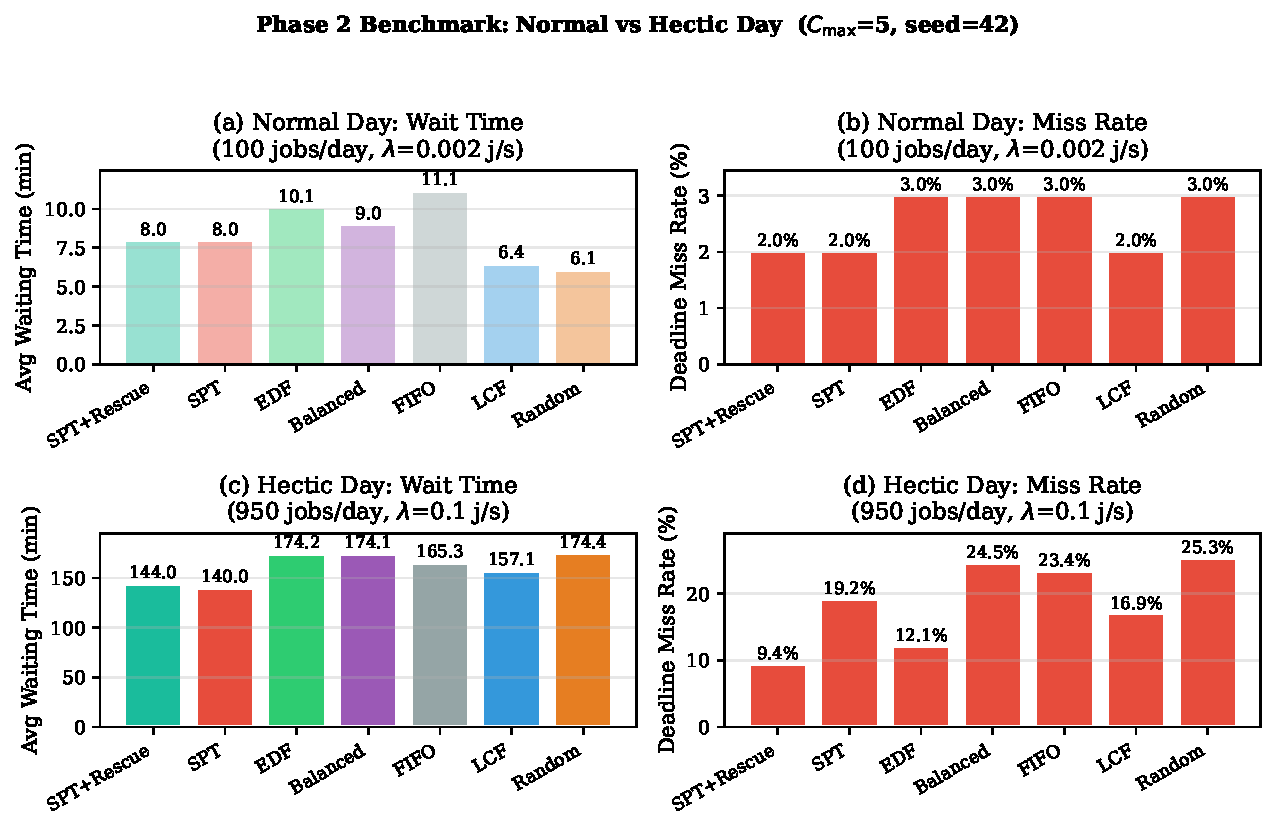
\includegraphics[width=0.98\linewidth,height=0.80\textheight,keepaspectratio]{figures/phase2_comparison.pdf}
\caption[Phase 2 benchmark: normal vs hectic day]{Phase 2 benchmark: normal vs hectic day.}
\label{fig:phase2}
\end{figure}
\end{landscape}

\noindent\textit{Figure~\ref{fig:phase2} notes.} Phase 2 benchmark results ($C_{\max}=5$, seed=42, 20\% tight 1h / 80\% loose 8h deadlines). Top row: a normal day ($\sim$100 jobs/day, $\rho<1$), where all schedulers achieve near-zero miss and wait under about 12~minutes, confirming that scheduler choice is immaterial under light load. Bottom row: the hectic day ($\sim$950 jobs/day, $\lambda=0.100$ j/s; capacity saturation), the discriminating regime analysed below. In this seed SPT+Rescue records the lowest miss (\PhTwoRescueMiss\%, at \PhTwoRescueWait~min wait) and SPT the lowest wait (\PhTwoSPTwait~min) of the seven baseline schedulers; SPT's miss (\PhTwoSPTmiss\%) is about twice SPT+Rescue's; EDF's miss (\PhTwoEDFmiss\%) is lower here than its 30-seed Phase~3 mean, illustrating single-seed variance under saturation; FIFO, LCF, and Balanced ignore deadlines, and FIFO's miss (\PhTwoFIFOmiss\%) is high but not the highest of the seven in this seed (Balanced and Random are higher).\par

Four observations follow from Phase~2, though as a single seed it carries no confidence interval and several of the following patterns do not survive to the robust $n=30$ Phase~3 mean; that comparison is made explicit below. First, in this seed SPT has the lowest waiting time (\PhTwoSPTwait~min) and SPT+Rescue the lowest miss rate (\PhTwoRescueMiss\%) of the seven baseline schedulers, with SPT+Rescue's wait four minutes higher (\PhTwoRescueWait~min): the laxity rescue mechanism trades a little wait for a large miss reduction on this particular seed, the same direction as the $n=30$ result (Section~\ref{sec:phase-3-statistical-validation}), where SPT and RH have no significant paired wait difference and form the lowest-wait tier and SPT+Rescue trails both; the single seed nevertheless shows a larger gap than the mean, which is why Phase~3's 30-seed replication, not this single seed, is the basis for every inferential claim in this thesis. Second, SPT's miss rate in this seed (\PhTwoSPTmiss\%) is about twice that of SPT+Rescue, a larger ratio than at $n=30$, consistent with shortest-job-first ordering sacrificing tight-deadline jobs under saturation. Third, EDF's miss rate in this seed (\PhTwoEDFmiss\%) is lower than its Phase~3 mean of \EDFmiss\% ($n=30$), reflecting high seed-to-seed variance under saturation, so the Phase~3 result provides the reliable cross-seed estimate rather than this seed's draw. Fourth, FIFO processes jobs without deadline awareness and has a high miss rate (\PhTwoFIFOmiss\%), though in this seed Balanced and Random are worse on miss: under saturation, a large fraction of tight-deadline jobs fail to complete within 1 hour. Across all policies, the schedulers achieve \PhTwoUtilPct\% event-sampled concurrency utilisation and 100\% job completion (all 950 jobs dispatched); the utilisation figure is the mean of per-event samples, which concentrate on the busy active window, and is not a time-weighted average over the full 24-hour day, most of which lies after the backlog drains.

\section{Phase 3 Statistical Validation}
\label{sec:phase-3-statistical-validation}

Table~\ref{tab:statistical} reports Phase~3 results over $n=30$ seeds on hectic-day workload (configuration in Section~\ref{ssec:platform-and-data}), with 95\% confidence intervals. Figure~\ref{fig:phase3-ci} plots the same intervals graphically, showing each scheduler's own across-seed spread; because the schedulers share seeds, overlap of these marginal intervals is not a test of any pair, and the paired mean differences and tests in Table~\ref{tab:ttests} give the verdict for the pairs compared there.

\begin{table}[htbp]
\centering
\caption[Phase 3 statistical validation]{Phase 3 statistical validation: $n=30$ seeds, hectic day ($C_{\max}=5$, $\sim$950 jobs/day, $\lambda=0.100$ j/s, 20\% tight 1h / 80\% loose 8h deadlines; capacity saturation $\rho>1$)}
\label{tab:statistical}
\resizebox{\linewidth}{!}{\begin{tabular}{lrrrrrr}
\toprule
\textbf{Scheduler} & \textbf{Avg Wait (min)} & \textbf{95\% CI} & \textbf{Miss \%} & \textbf{95\% CI} & \textbf{Avg Tardiness (min)} & \textbf{Cost (\$)} \\
\midrule
\textbf{RH} & 141.70 & [137.90,~145.50] & \textbf{9.60} & [8.41,~10.78] & 31.84 & 6.35\\
CADR & 144.66 & [141.35,~147.97] & 9.68 & [8.18,~11.18] & 5.95 & 6.36\\
SPT+Rescue & 146.32 & [143.28,~149.36] & 13.56 & [12.45,~14.68] & 5.89 & 6.37\\
Adaptive & 169.67 & [165.97,~173.36] & 12.62 & [11.08,~14.16] & 4.91 & 6.39\\
\textbf{SPT} & \textbf{141.45} & [137.52,~145.38] & 18.96 & [17.26,~20.67] & 12.02 & 6.34\\
EDF & 170.22 & [166.99,~173.45] & 14.71 & [13.28,~16.13] & 5.16 & 6.41\\
LCF & 166.91 & [164.03,~169.79] & 24.24 & [22.97,~25.51] & 25.25 & 6.37\\
Balanced & 168.59 & [165.50,~171.69] & 25.25 & [24.18,~26.31] & 26.66 & 6.38\\
FIFO & 167.93 & [164.10,~171.75] & 24.43 & [23.14,~25.72] & 26.01 & 6.40\\
Random & 167.68 & [164.62,~170.74] & 23.44 & [22.64,~24.24] & 32.89 & 6.38\\
\bottomrule
\end{tabular}
}
\end{table}

\begin{figure}[htbp]
\centering
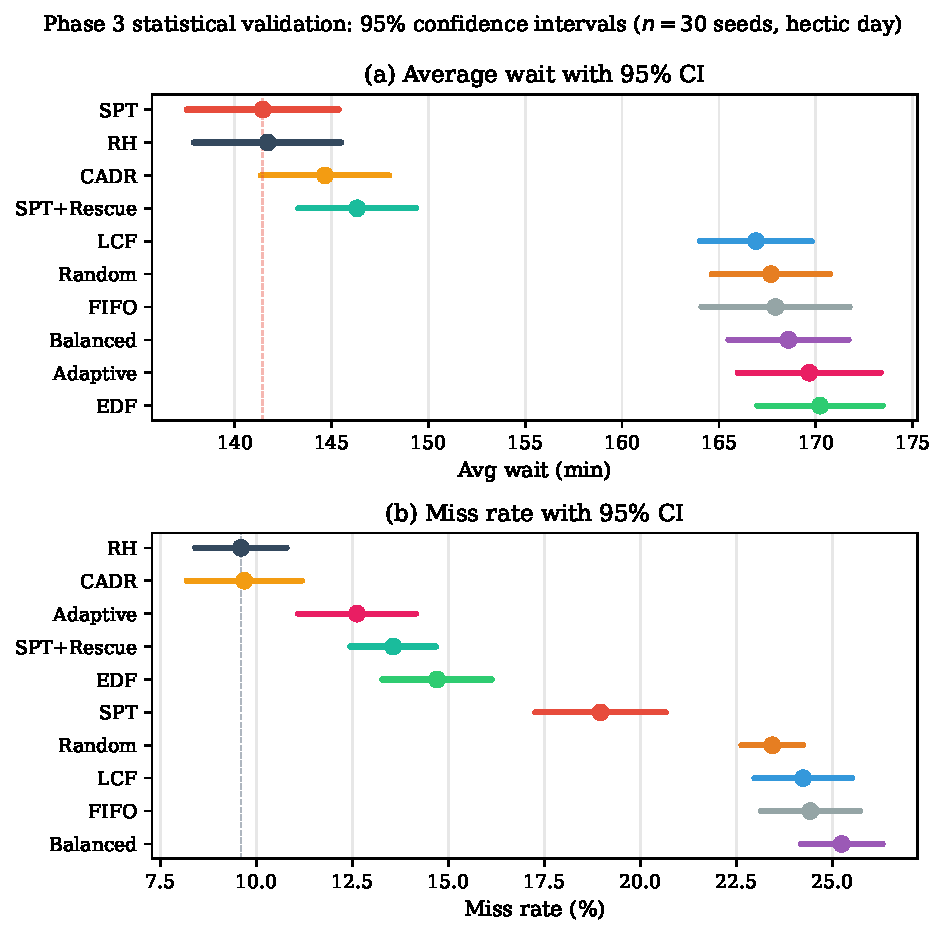
\includegraphics[width=0.97\textwidth]{figures/phase3_ci.pdf}
\caption[Phase 3: 95\% confidence intervals]{Phase 3 confidence interval plot: 95\% CIs for average wait (a) and miss rate (b) for all ten schedulers, $n=30$ seeds, hectic day. Schedulers are ordered by mean value within each panel. These are marginal intervals summarising each scheduler's own across-seed variability, so they describe the spread of the ten distributions and are not themselves a test of any pair. Because every scheduler is run on the same 30 seeds (a randomised block design, Section~\ref{ssec:statistical-methodology}), the paired tests of Table~\ref{tab:ttests} are the authoritative verdict, and overlap here need not agree with them in either direction: EDF's and FIFO's wait intervals overlap although that pair separates at the uncorrected level, and EDF's and SPT's miss intervals overlap by a hair although the paired test separates them clearly ($p<0.001$). Key groupings: RH and CADR have the lowest miss point estimates, with no significant paired difference (paired $t=\RHCADRmissT$, $p=\RHCADRmissP$; this does not establish equivalence); SPT and RH are tied for the lowest wait (paired $t=\RHSPTwaitT$, $p=\RHSPTwaitP$); EDF achieves significantly lower miss than SPT despite much higher wait, underscoring that deadline-awareness and throughput are separate design levers.}
\label{fig:phase3-ci}
\end{figure}

\begin{figure}[H]
\centering
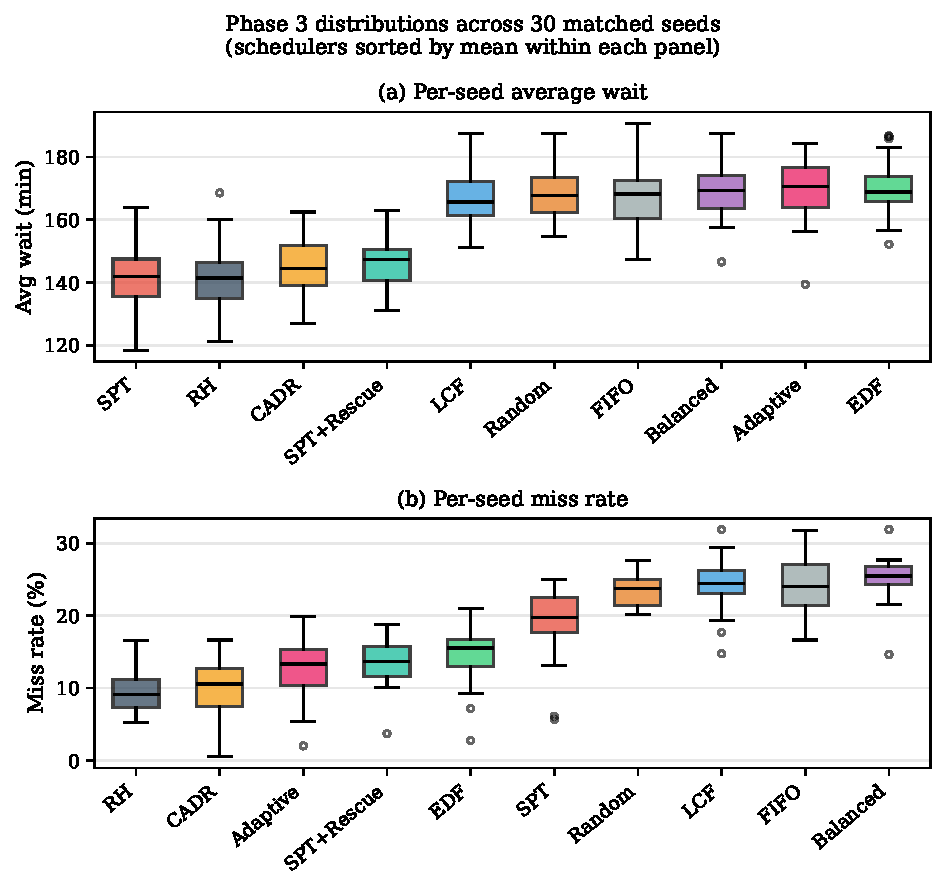
\includegraphics[width=0.97\textwidth]{figures/seed_distributions.pdf}
\caption[Phase 3: per-seed distributions]{Per-seed distributions behind the Phase 3 means: box plots of average wait (a) and miss rate (b) across the 30 matched seeds, schedulers sorted by mean within each panel. The box spans the interquartile range with the median line; whiskers extend to 1.5$\times$IQR and dots mark outlier seeds. The clear vertical separation between the deadline-aware and deadline-oblivious groups in panel~(b) holds seed by seed, not just on average, which is what the paired tests in Table~\ref{tab:ttests} formalise.}
\label{fig:seed-distributions}
\end{figure}

Figure~\ref{fig:seed-distributions} complements the interval view with the full per-seed distributions, showing that the group separations hold across individual seeds rather than only in the aggregate. Table~\ref{tab:ttests} reports the pairwise paired $t$-test results.

\begin{table}[htbp]
\centering
\caption[Pairwise paired t-test results]{Pairwise paired $t$-test results, Phase 3 ($n=30$, $C_{\max}=5$, hectic day $\sim$950 jobs/day, 20\% tight 1h / 80\% loose 8h deadlines). Each comparison is matched on seed; a Wilcoxon signed-rank test gives raw $p<0.05$ for every entry marked significant. ``Significant?'' reflects the Holm-Bonferroni-corrected verdict at family-wise $\alpha=0.05$ (Section~\ref{ssec:statistical-methodology}), not the raw uncorrected $p$-value; $^\dagger$marks the two comparisons whose raw $p<0.05$ but which do not survive the correction. Mean differences are first-named minus second-named scheduler (minutes for wait, percentage points for miss), with a paired $t$-based 95\% confidence interval ($\mathrm{df}=29$) that is unadjusted for multiplicity, so the two $^\dagger$ rows exclude zero at the raw level while failing the Holm-corrected test.}
\label{tab:ttests}
\small
\resizebox{\textwidth}{!}{%
\begin{tabular}{llrrlrr}
\toprule
\textbf{Comparison} & \textbf{Metric} & $t$ & $p$-value & \textbf{Significant?} & Mean diff.\ [95\% CI] & Cohen's $d$ \\
\midrule
SPT vs FIFO        & Avg wait   & $\SPTFIFOwaitT$    & $<0.001$           & Yes & $\SPTFIFOwaitMD$ [$\SPTFIFOwaitMDLo$, $\SPTFIFOwaitMDHi$] & $\SPTFIFOwaitD$ \\
SPT vs FIFO        & Miss rate  & $\SPTFIFOmissT$    & $<0.001$           & Yes & $\SPTFIFOmissMD$ [$\SPTFIFOmissMDLo$, $\SPTFIFOmissMDHi$] & $\SPTFIFOmissD$ \\
SPT+Rescue vs FIFO & Avg wait   & $\RescueFIFOwaitT$ & $<0.001$           & Yes & $\RescueFIFOwaitMD$ [$\RescueFIFOwaitMDLo$, $\RescueFIFOwaitMDHi$] & $\RescueFIFOwaitD$ \\
SPT+Rescue vs FIFO & Miss rate  & $\RescueFIFOmissT$ & $<0.001$           & Yes & $\RescueFIFOmissMD$ [$\RescueFIFOmissMDLo$, $\RescueFIFOmissMDHi$] & $\RescueFIFOmissD$ \\
EDF vs FIFO        & Avg wait   & $\EDFFIFOwaitT$    & $\EDFFIFOwaitP$    & No  & $\EDFFIFOwaitMD$ [$\EDFFIFOwaitMDLo$, $\EDFFIFOwaitMDHi$] & $\EDFFIFOwaitD$ \\
EDF vs FIFO        & Miss rate  & $\EDFFIFOmissT$    & $<0.001$           & Yes & $\EDFFIFOmissMD$ [$\EDFFIFOmissMDLo$, $\EDFFIFOmissMDHi$] & $\EDFFIFOmissD$ \\
Random vs FIFO     & Miss rate  & $\RandomFIFOmissT$ & $\RandomFIFOmissP$ & No$^\dagger$ & $\RandomFIFOmissMD$ [$\RandomFIFOmissMDLo$, $\RandomFIFOmissMDHi$] & $\RandomFIFOmissD$ \\
SPT vs EDF         & Miss rate  & $+\SPTEDFmissT$    & $<0.001$          & Yes & $+\SPTEDFmissMD$ [$\SPTEDFmissMDLo$, $\SPTEDFmissMDHi$] & $+\SPTEDFmissD$ \\
RH vs FIFO          & Avg wait   & $\RHFIFOwaitT$   & $<0.001$ & Yes & $\RHFIFOwaitMD$ [$\RHFIFOwaitMDLo$, $\RHFIFOwaitMDHi$] & $\RHFIFOwaitD$ \\
RH vs FIFO          & Miss rate  & $\RHFIFOmissT$   & $<0.001$ & Yes & $\RHFIFOmissMD$ [$\RHFIFOmissMDLo$, $\RHFIFOmissMDHi$] & $\RHFIFOmissD$ \\
RH vs SPT+Rescue    & Avg wait   & $\RHRescueWaitT$ & $\RHRescueWaitP$ & No$^\dagger$ & $\RHRescueWaitMD$ [$\RHRescueWaitMDLo$, $\RHRescueWaitMDHi$] & $\RHRescueWaitD$ \\
RH vs SPT+Rescue    & Miss rate  & $\RHRescueMissT$ & $<0.001$ & Yes & $\RHRescueMissMD$ [$\RHRescueMissMDLo$, $\RHRescueMissMDHi$] & $\RHRescueMissD$ \\
RH vs CADR          & Miss rate  & $\RHCADRmissT$   & $\RHCADRmissP$ & No  & $\RHCADRmissMD$ [$\RHCADRmissMDLo$, $\RHCADRmissMDHi$] & $\RHCADRmissD$ \\
\bottomrule
\end{tabular}}
\end{table}

\begin{landscape}
\begin{figure}[H]
\centering
\captionsetup{font=small,skip=6pt}
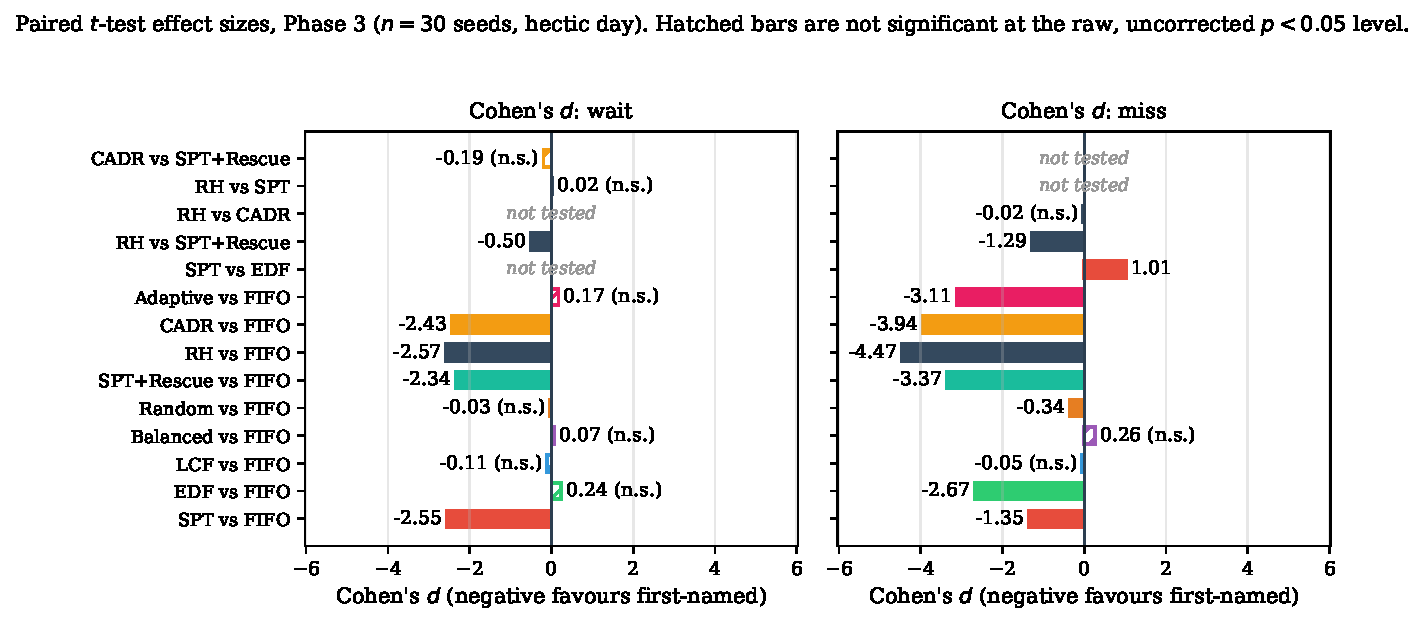
\includegraphics[width=0.98\linewidth,height=0.72\textheight,keepaspectratio]{figures/ttest_effects.pdf}
\caption[Paired t-test effect sizes]{Effect sizes for the whole pairwise family, of which Table~\ref{tab:ttests} prints the pre-specified subset: Cohen's $d$ for average wait (left) and miss rate (right). Negative bars favour the first-named scheduler; hatched bars are not significant at the raw, uncorrected $p<0.05$ level, and pairs without a pre-specified hypothesis for a metric are marked ``not tested''. The headline RH vs CADR miss comparison is non-significant on the paired test, without establishing equivalence, while RH vs FIFO shows the largest miss effect in the study. The shading is the uncorrected verdict, so \HolmRemoved{} bars render solid without surviving the Holm-Bonferroni family-wise correction: RH's wait advantage over SPT+Rescue ($d=\RHRescueWaitD$, raw $p=\RHRescueWaitP$) and Random's lower miss than FIFO ($d=\RandomFIFOmissD$, raw $p=\RandomFIFOmissP$). Defer to the table, not this figure, for every corrected verdict.}
\label{fig:ttest-effects}
\end{figure}
\end{landscape}

Figure~\ref{fig:ttest-effects} presents the same comparisons graphically. The $p$-values are computed from the exact Student $t$-distribution for the paired differences ($\mathrm{df}=n-1$), so they match an independent recomputation (\texttt{scipy.stats.ttest\_rel}); a Wilcoxon signed-rank test gives raw $p<0.05$ for every Holm-significant result, so the conclusions are not artefacts of the normality assumption. Applying the same Holm step-down to the Wilcoxon $p$-values leaves \WilcoxHolmNSig{} of the \HolmNSig{}, so the distribution-free test agrees with the $t$-test family on which comparisons survive. The full pairwise family comprises \HolmFamily{} comparisons, of which Table~\ref{tab:ttests} prints the pre-specified subset; the Holm-Bonferroni step-down correction is applied over the whole family, not over the printed rows, to control the family-wise error rate. Of the \HolmUncorrSig{} comparisons significant at the uncorrected $0.05$ level, \HolmNSig{} remain significant after the correction (the largest surviving $p$-value is below $0.001$), so the correction removes \HolmRemoved{} of them. Both are printed in Table~\ref{tab:ttests} and marked with $^\dagger$ rather than reported as headline findings: RH's wait advantage over SPT+Rescue, and Random's lower miss than FIFO. The wait difference between EDF and FIFO, and the LCF and Balanced comparisons against FIFO, are not significant even before correction, and no claim about any of them is made in this thesis beyond that. Tests reported elsewhere in this chapter are neither members of this family nor included in these counts, and are stated uncorrected. That applies in particular to the three significant tests drawn from the availability and prior sweeps (Section~\ref{ssec:availability-model-sensitivity}), each of which carries a $p$-value well below the smallest threshold a correction over a family of this size could impose, so no conclusion drawn from them turns on the distinction.

The statistical comparison supports the following conclusions.

SPT achieves the lowest wait among the baseline policies under capacity saturation, with no significant paired wait difference from RH. Under hectic overload ($\sim$950 jobs, $\rho>1$), SPT achieves the lowest baseline wait (RH's mean is marginally higher, and the paired test over the same 30 seeds cannot separate the two: $t=\RHSPTwaitT$, $p=\RHSPTwaitP$, $d=\RHSPTwaitD$) but is now significantly outperformed by EDF on miss (\SPTmiss\% vs \EDFmiss\%, $d=\SPTEDFmissD$, $p<0.001$): the two are no longer statistically tied on miss. The effect vs FIFO is large on both metrics.

SPT+Rescue achieves a notably lower miss rate than SPT (\RescueMiss\% vs \SPTmiss\%) but at higher wait (\RescueWait~min vs \SPTwait~min). Under full saturation ($\rho>1$), the rescue tier reorders urgent jobs ahead of the normal SPT queue but cannot prevent all misses caused by the $C_{\max}=5$ concurrency ceiling; promoting urgent jobs displaces normal-tier jobs, adding wait while still reducing net miss relative to bare SPT. The lower mean miss also yields a larger Cohen's $d$ vs FIFO ($d=\RescueFIFOmissD$) than bare SPT ($d=\SPTFIFOmissD$), even though SPT+Rescue's miss rate varies more across seeds than SPT's. SPT+Rescue still provides a very large improvement over FIFO/LCF/Balanced on both metrics.

EDF now achieves significantly lower miss than SPT ($d=\SPTEDFmissD$, $p<0.001$) and carries a higher mean wait than FIFO that the paired test does not resolve ($d=\EDFFIFOwaitD$, $p=\EDFFIFOwaitP$): its deadline ordering helps on miss, while reordering the queue around deadlines rather than job length buys no wait advantage at all over the deadline-oblivious baseline. EDF's mean tardiness (\EDFtard~min) remains low relative to the deadline-oblivious policies, though it no longer leads the deadline-aware group: the Adaptive hybrid now posts lower tardiness (\AdaptiveTard~min vs \EDFtard~min), while CADR (\CADRtard~min) and SPT+Rescue (\RescueTard~min) sit just above EDF (Section~\ref{sec:ablation-analysis}).

RH has the lowest miss-rate point estimate under hectic saturation (\RHMiss\%, with no significant paired difference from CADR's in the 30-seed test, as shown below) while its mean wait (\RHWait~min) is in the lowest tier, with no significant paired wait difference from SPT (\SPTwait~min; $t=\RHSPTwaitT$, $p=\RHSPTwaitP$) and numerically lower than SPT+Rescue (\RescueWait~min). RH's miss advantage over SPT+Rescue survives Holm correction ($d=\RHRescueMissD$, $p<0.001$); its wait advantage, while numerically favourable, has a raw $p=\RHRescueWaitP$ that does \emph{not} survive the family-wise correction (Table~\ref{tab:ttests}), so RH is best described as significantly better than SPT+Rescue on miss and comparable to it on wait, rather than dominant on both metrics. Versus FIFO both gaps are large and significant (miss $d=\RHFIFOmissD$, wait $d=\RHFIFOwaitD$, both $p<0.001$), and RH's operational cost is within roughly 1\% of SPT+Rescue (Section~\ref{ssec:objective-weight-sensitivity}). RH's mean tardiness (\RHtard~min) is not only substantially higher than EDF's (\EDFtard~min) but now exceeds even the deadline-oblivious FIFO baseline (\FIFOtard~min): its urgent tier promotes a tight job only in roughly the last service time before its deadline, and a tight job that misses that window is demoted behind the loose backlog, so under this workload the jobs RH misses are missed by more than FIFO's, even though RH misses far fewer jobs overall.

CADR achieves near-RH miss (\CADRmiss\%) while cutting RH's mean tardiness by \CADRtardReduction\% (\CADRtard~min vs \RHtard~min). CADR's critical-ratio triage promotes at-risk jobs earlier than RH's urgent tier (at $\mathrm{CR}_j \leq 3$ rather than only when a job cannot wait for the next slot), so fewer tight jobs fall into the demoted tier and its misses are mostly loose jobs finishing modestly late. At Phase~3 hectic load, CADR has a lower miss point estimate than SPT+Rescue (\CADRmiss\% vs \RescueMiss\%; no paired miss test between them is in the pre-specified family) at a wait the paired test cannot separate (\CADRwait~min vs \RescueWait~min; $t=\CADRRescueWaitT$, $p=\CADRRescueWaitP$, $d=\CADRRescueWaitD$) and comparable tardiness (\CADRtard~min vs \RescueTard~min): CADR's advantage over SPT+Rescue is concentrated on miss rate rather than a joint improvement on both QoS metrics. The paired RH--CADR miss comparison is not significant ($t=\RHCADRmissT$, $p=\RHCADRmissP$; RH \RHMiss\% vs CADR \CADRmiss\%). Its 95\% interval for the RH-minus-CADR difference is [\RHCADRmissMDLo, \RHCADRmissMDHi] percentage points, so it does not establish equivalence; the choice between the two proposed schedulers can also consider tardiness: RH holds the lower miss point estimate, while CADR has substantially lower mean lateness. Given the unresolved baseline miss difference and CADR's lower tardiness, CADR is the recommended default. RH's miss lead is a point estimate at baseline, becomes significant only at the scarcer $\times 0.75$ availability scale, and reverses under the eased and data-ordered availability settings (Section~\ref{ssec:availability-model-sensitivity}), so RH is the specialist for the scarce baseline regime when the lowest miss count is what matters. For operators who prioritise queue wait, SPT is the natural choice (tied with RH at the hectic baseline and lower elsewhere); RH's wait edge over CADR is an untested point estimate.

The Adaptive queue-pressure EDF-SPT hybrid lands in the mid-tier (\AdaptiveMiss\% miss, \AdaptiveWait~min wait, \AdaptiveTard~min tardiness). Its queue-pressure rule widens the urgent tier to every positive-laxity job once the backlog exceeds the pressure threshold $P$, so at any scheduling event with more than $P$ queued jobs it orders nonnegative-laxity jobs by deadline with hopeless demotion. This betters plain EDF (\EDFmiss\%) and SPT (\SPTmiss\%) on miss and sits about one percentage point below SPT+Rescue (\RescueMiss\%), a gap that no pre-specified test in this study addresses; its mean wait sits slightly above FIFO's rather than matching it, because EDF ordering carries no throughput benefit. CADR has lower miss and wait point estimates than Adaptive at comparable cost (the miss gap is borderline and uncorrected, outside the pre-specified family), though Adaptive holds the lowest mean tardiness of all ten policies (\AdaptiveTard~min), confirming that the adaptive SPT-EDF hybrid design is sound but the proposed RH and CADR policies are stronger on the primary QoS metrics.

Finally, FIFO, LCF, and Balanced incur the highest miss rates. These schedulers carry no deadline information; under saturation tight-deadline jobs queued behind loose-deadline jobs routinely miss their 1-hour window.

\section{Ablation Analysis}
\label{sec:ablation-analysis}

Table~\ref{tab:ablation} traces the evolutionary chain FIFO $\to$ SPT $\to$ SPT+Rescue $\to$ RH on Phase~3 hectic-day results ($n=30$ seeds), showing how each algorithmic addition changes waiting time, deadline miss rate, and mean tardiness relative to the previous step. EDF is included as an alternative single-criterion branch off FIFO (a deadline-driven sibling of the shortest-job-first SPT), isolating which design ingredient, shortest-job-first ordering or deadline awareness, drives each metric. CADR and the CADR-order-only (CADR-OO) ablation variant are included to show the contribution of the cost-aware placement component, and the Adaptive queue-pressure EDF-SPT hybrid is included as an alternative hybrid branch. Cohen's $d$ is computed against FIFO for every row except SPT+Rescue, which is compared with SPT (the step-wise RH versus SPT+Rescue effect is in Table~\ref{tab:ttests}): positive $d$ indicates an increase (worse) relative to the comparison policy, negative $d$ indicates a decrease (better). Figure~\ref{fig:ablation-waterfall} plots the three metrics across the chain, making the per-step trade-offs visible at a glance.

\begin{table}[htbp]
\centering
\caption[Ablation analysis: evolutionary chain]{Ablation analysis: evolutionary chain on Phase~3 hectic day ($n=30$ seeds, $C_{\max}=5$, $\sim$950 jobs/day). Cohen's $d$ for SPT, EDF, RH, CADR, and Adaptive is relative to FIFO; for SPT+Rescue it is relative to SPT. The RH and CADR comparisons against SPT+Rescue are reported in Table~\ref{tab:ttests} and the Phase~3 statistics (Section~\ref{sec:phase-3-statistical-validation}).}
\label{tab:ablation}
\resizebox{\linewidth}{!}{\begin{tabular}{lrrrrr}
\toprule
\textbf{Scheduler} & \textbf{Avg Wait (min)} & \textbf{Miss \%} & \textbf{Avg Tardiness (min)} & \textbf{Cohen $d$ (wait)} & \textbf{Cohen $d$ (miss)} \\
\midrule
FIFO & 167.93 & 24.43 & 26.01 & -- & -- \\
SPT & 141.45 & 18.96 & 12.02 & -2.552 & -1.351 \\
EDF & 170.22 & 14.71 & 5.16 & 0.242 & -2.668 \\
SPT+Rescue & 146.32 & 13.56 & 5.89 & 0.518 & -1.402 \\
\textbf{RH} (proposed) & 141.70 & 9.60 & 31.84 & -2.571 & -4.467 \\
\textbf{CADR} (proposed) & 144.66 & 9.68 & 5.95 & -2.430 & -3.936 \\
Adaptive (EDF-SPT hybrid) & 169.67 & 12.62 & 4.91 & 0.173 & -3.109 \\
\midrule
CADR-order-only & 145.96 & 10.16 & 6.59 & -- & -- \\
\bottomrule
\end{tabular}
}
\end{table}

\begin{landscape}
\begin{figure}[H]
\centering
\captionsetup{font=small,skip=6pt}
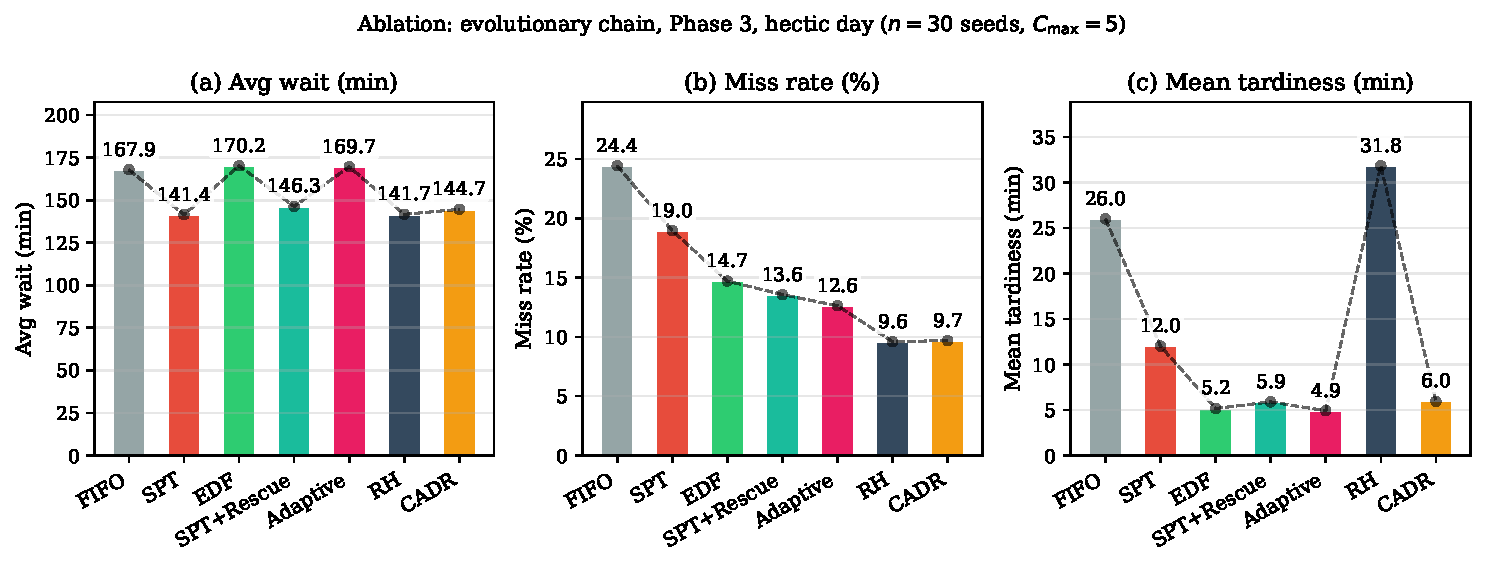
\includegraphics[width=0.98\linewidth,height=0.72\textheight,keepaspectratio]{figures/ablation_waterfall.pdf}
\caption[Ablation waterfall across the design chain]{Ablation waterfall: average wait (a), miss rate (b), and mean tardiness (c) for each scheduler in the evolutionary chain. Each step along the chain adds one algorithmic ingredient. SPT improves both wait and miss over FIFO; EDF cuts miss and tardiness but leaves wait at FIFO level; SPT+Rescue recovers deadline awareness while retaining most of SPT's wait advantage; the Adaptive hybrid (plotted alongside the main chain) widens the rescue idea's urgent tier under queue pressure, with a miss rate slightly below SPT+Rescue's at EDF-like tardiness, though its wait reverts to FIFO level; RH then improves miss significantly and wait numerically over SPT+Rescue (the wait gain does not survive Holm correction), at the price of high tardiness on the jobs it sacrifices; CADR trades a marginal wait increase for a large tardiness reduction (\RHtard{} to \CADRtard\,min) at near-identical miss.}
\label{fig:ablation-waterfall}
\end{figure}
\end{landscape}

The ablation chain isolates the contribution of each design ingredient. The first step, SPT over FIFO, shows that shortest-job-first ordering produces a large reduction in waiting time ($d$ vs FIFO from Table~\ref{tab:ttests}) and a statistically significant miss reduction, confirming that shortest-job-first ordering benefits both metrics simultaneously under saturation. The alternative branch, EDF over FIFO, shows that pure earliest-deadline ordering cuts the miss rate even more than SPT does ($d=\EDFFIFOmissD$ vs $d=\SPTFIFOmissD$) but leaves waiting time at or slightly above FIFO's ($d=\EDFFIFOwaitD$, $p=\EDFFIFOwaitP$, not significant even before correction). Contrasting the EDF and SPT branches therefore isolates the two design ingredients: deadline awareness alone is sufficient to reduce misses under saturation, whereas the wait-time benefit comes specifically from shortest-job-first ordering. This motivates the hybrid designs, which seek both effects at once. EDF's mean tardiness (\EDFtard~min) remains low relative to the deadline-oblivious policies, because its deadline ordering ensures even missed jobs are missed by a small amount, though it no longer leads the deadline-aware group on this metric (the Adaptive hybrid posts lower tardiness here, \AdaptiveTard~min, while CADR and SPT+Rescue sit just above EDF).

The step from SPT to SPT+Rescue shows that the laxity rescue mechanism cuts the mean miss rate substantially (\RescueMiss\% vs \SPTmiss\%, reflected in a larger Cohen $d$ vs FIFO of \RescueFIFOmissD{} against \SPTFIFOmissD{} for SPT), although its miss rate varies more across seeds than SPT's, and it increases mean waiting time because urgent-tier promotions displace short normal-tier jobs. The step from SPT+Rescue to RH improves miss significantly and wait numerically (Table~\ref{tab:ttests}: $d=\RHRescueWaitD$ wait, which does not survive Holm correction, $d=\RHRescueMissD$ miss vs SPT+Rescue); plain SPT also improves both relative to FIFO, but at a far higher miss level. Replacing the fixed laxity threshold with timeline-derived urgency restores SPT shortest-job-first ordering for jobs with slack, cutting wait back to SPT-level; simultaneously, hopeless-demotion (demoting jobs projected to miss under the mean-service estimate in favour of jobs projected to meet their deadlines) combined with precise forward-simulation urgency cuts miss below SPT+Rescue's fixed-threshold approach. However, RH's late promotion of tight jobs, which then fall into its demoted tier, increases mean tardiness relative to SPT+Rescue (\RHtard~min vs \RescueTard~min): jobs that are pushed to the back are missed by substantially more.

CADR at Phase~3 hectic load has a lower miss point estimate than SPT+Rescue (\CADRmiss\% vs \RescueMiss\%; no paired miss test is in the pre-specified family) at essentially the same wait (\CADRwait~min vs \RescueWait~min) and comparable tardiness (\CADRtard~min vs \RescueTard~min); the advantage over SPT+Rescue is concentrated on miss rate rather than a joint improvement on both metrics. CADR achieves near-RH miss (\CADRmiss\% vs \RHMiss\%) while cutting RH's mean tardiness substantially (\CADRtard~min vs \RHtard~min), because its critical-ratio triage promotes at-risk jobs earlier, so fewer tight jobs are demoted behind the loose backlog. RH retains the lowest miss point estimate, though not significantly below CADR's. These are complementary designs, not a linear ``each step better'' chain; because the paired baseline miss test does not separate them and CADR's missed jobs are far less late, CADR is the recommended default and RH the specialist for the scarce baseline regime (Section~\ref{ssec:choosing-between-rh-and-cadr}).

The CADR-order-only (CADR-OO) ablation retains the three-tier critical-ratio ordering but replaces cost-aware node selection with fastest-available-node placement, yielding \CADROOmiss\% miss and \CADROOtard~min tardiness, vs CADR's \CADRmiss\% and \CADRtard~min. Removing cost-aware placement therefore makes no detectable difference to QoS (\CADROOmiss\% vs \CADRmiss\% on miss, and \CADROOtard~min vs \CADRtard~min on tardiness, all within seed-to-seed noise, with tardiness marginally lower without it). This is expected: operational cost headroom is structurally small in this fleet (a marginal, near-noise gap across policies), so optimising node selection for cost does not move the QoS metrics, and CADR's QoS comes from its critical-ratio ordering.

Lastly, the Adaptive queue-pressure hybrid achieves lower miss (\AdaptiveMiss\%) than pure EDF (\EDFmiss\%) and about one percentage point below SPT+Rescue (\RescueMiss\%), with EDF-like low tardiness (\AdaptiveTard~min). These observed results place Adaptive below both SPT+Rescue and EDF on miss point estimate, but no pressure-rule ablation isolates how much of that difference comes from tier widening. It has higher miss and wait point estimates than both proposed schedulers, with no paired test between them: RH (\RHMiss\% miss) and CADR (\CADRmiss\% miss). Tardiness runs the other way, with Adaptive lowest of the ten (\AdaptiveTard~min). The observed miss point estimates put the two proposed schedulers below Adaptive on this workload; the contribution of Adaptive's pressure rule remains unisolated.


\subsection{Capacity Lower Bound}
\label{ssec:capacity-lower-bound}

To situate the Phase~3 miss rates against what any policy could achieve, two brackets are computed on the expected-service hectic instances (the same 30 job streams, each job granted its fastest GPU's mean execution time and zero provisioning delay). First, a certified window-capacity bound: for any window $[s,t]$, the jobs submitted at or after $s$ with deadlines at or before $t$ must fit their total work into $C_{\max}(t-s)$ machine-seconds, so any excess implies unavoidable misses under \emph{every} policy, clairvoyant or not. Across all 30 seeds this bound certifies \CapBoundMeanPct\% unavoidable misses (maximum \CapBoundMaxMisses{} jobs in any seed): the tight-deadline stream alone never exceeds fleet capacity, and the loose eight-hour windows spread the remaining demand far below it. Second, a constructive clairvoyant relaxation: non-preemptive EDF with full hindsight on the same relaxed instances schedules every job on time in every seed (\RelaxEDFMeanPct\% miss). The certificate is one-sided and deterministic: it bounds the expected-service instance, not individual stochastic realisations, whose provisioning and service draws can and do produce misses; that residual is precisely what the simulator measures. The offline-relaxed optimum is therefore exactly zero misses, and no reachable-optimum gap can be quoted against it; instead, the observed miss rates measure the \emph{price of real operation}: online arrivals (Section~\ref{sec:computational-complexity}), non-preemptive dispatch on a heterogeneous fleet, stochastic provisioning delays, and stochastic service times. RH's \RHMiss\% is the smallest measured price among the ten policies as a point estimate (CADR's paired miss difference is not significant in the 30-seed test), and the concurrency study (Section~\ref{ssec:concurrency-limit-sensitivity}) shows RH's residual falling to about 2\% at $C_{\max}=7$ and reaching zero at $C_{\max}=10$, consistent with the relaxation's verdict that baseline capacity is sufficient in expectation. The computation is reproducible via \texttt{CGRSP/phase3\_capacity\_bound.py}.

\subsection{Classical and Learned Baselines}
\label{ssec:classical-and-learned-baselines}

The main comparison in Section~\ref{sec:phase-3-statistical-validation} uses the ten policies of Chapter~\ref{chap:system}. Five further baselines are run on the same 30 seeds, job count, arrival rate, concurrency limit and deadline split: HEFT, min-min, max-min, a shallow tabular bandit, and a uniform random-arm control for that bandit. For independent jobs, HEFT reduces to longest-average-job-first ordering with earliest-finish-time placement, and min-min repeatedly takes the job with the smallest earliest-completion time; both are described in Section~\ref{sec:heterogeneous-machine-scheduling}. The bandit selects among four arms (FIFO, SPT, EDF and SPT+Rescue), is trained for 15 episodes on seeds 500 to 514, and is evaluated with exploration switched off on seeds 0 to 29, so no evaluation seed appears in its training set. The random-arm control draws one of the same four arms uniformly at every decision. Table~\ref{tab:baselines} reports the three primary metrics.

\begin{table}[htbp]
\centering
\caption[Classical and learned baselines]{Classical and learned baselines on the Phase~3 hectic day ($n=30$ seeds, $\sim$950 jobs/day, $C_{\max}=5$, $\lambda=0.100$ j/s, 20\% tight 1h / 80\% loose 8h deadlines). HEFT and max-min produce identical values on every seed and every metric, so they are shown as one row. Mean tardiness is over completed jobs, with zero for on-time jobs. Bold marks the column minimum; the paired tests are in the text.}
\label{tab:baselines}
\begin{tabular}{lrrr}
\toprule
\textbf{Scheduler} & \textbf{Avg Wait (min)} & \textbf{Miss \%} & \textbf{Mean Tardiness (min)} \\
\midrule
HEFT $=$ MaxMin & 191.77 & 29.90 & 39.53\\
MinMin & \textbf{141.42} & 19.06 & 24.64\\
Bandit & 169.44 & 25.45 & 24.66\\
Bandit-random & 157.82 & 13.57 & \textbf{5.02}\\
FIFO & 167.93 & 24.43 & 26.01\\
RH & 141.70 & \textbf{9.60} & 31.84\\
CADR & 144.66 & 9.68 & 5.95\\
\bottomrule
\end{tabular}

\end{table}

The table separates the baselines sharply. HEFT and max-min are indistinguishable on this fleet: their per-seed values are identical on all six metrics, and the 30-comparison Holm family in the JSON therefore contains six duplicate comparisons, leaving 24 unique ones. HEFT's longest-average-job-first order is the reverse of SPT's, and max-min records the same values here; both record the highest wait (191.77~min) and miss rate (29.90\%) in the table, well above FIFO's \FIFOwait~min and \FIFOmiss\%.

MinMin records the lowest wait point estimate in the table (141.42~min). The paired test does not separate it from RH's \RHWait~min ($p_{\text{Holm}}=0.8904$, $d=-0.0283$), and its difference from CADR's \CADRwait~min is not significant at the raw or corrected level ($p=0.0831$, $p_{\text{Holm}}=0.3326$). Its miss rate is 19.06\%, however, significantly worse than RH's \RHMiss\% ($d=+2.4006$) and CADR's \CADRmiss\% ($d=+2.1770$), each $p<0.001$ after correction. MinMin therefore reaches the proposed schedulers on wait but not on deadline compliance.

The shallow bandit is a null result in this design. Its miss rate is 25.45\% against FIFO's \FIFOmiss\% ($p=0.1213$), and its wait is 169.44~min against \FIFOwait~min ($p=0.3383$); neither difference is significant, while RH and CADR are both significantly better than it on miss ($p<0.001$). The uniform random-arm control records a lower miss rate than the trained bandit (13.57\% against 25.45\%), so this experiment provides no evidence that the learned arm selection improves on chance. The result is specific to a tabular, episode-level bandit with four arms and a shallow training budget on this workload; it is not evidence about deep reinforcement learning, which remains open (Chapter~\ref{chap:conclusion}).

\section{Sensitivity Analysis}
\label{sec:sensitivity-analysis}

\subsection{Day-Type Sensitivity (\texorpdfstring{$C_{\max}=5$}{Cmax=5})}
\label{ssec:day-type-sensitivity-c-max-5}

Table~\ref{tab:sensitivity} summarises the average waiting time and deadline miss rate for all schedulers across four operationally calibrated day types at $C_{\max}=5$ (30 seeds per day type). Figure~\ref{fig:sensitivity} shows the full results. This study uses full 30-seed replication at every day type, matching the Phase~3 hectic-day protocol (Section~\ref{sec:phase-3-statistical-validation}); the surge-day anticipation benefit is additionally isolated at $n=30$ in the dedicated reservation study (Section~\ref{ssec:anticipation-reservation-sensitivity}).

\begin{landscape}
\begin{figure}[H]
\centering
\captionsetup{font=small,skip=6pt}
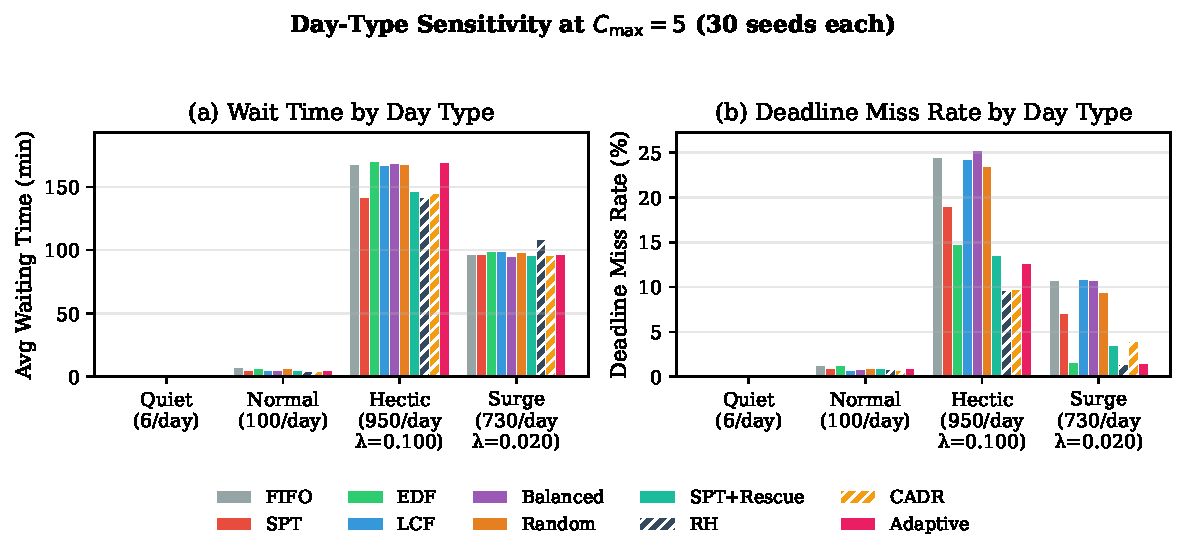
\includegraphics[width=0.98\linewidth,height=0.72\textheight,keepaspectratio]{figures/sensitivity_heatmap.pdf}
\caption[Day-type sensitivity results]{Day-type sensitivity at $C_{\max}=5$ (30 seeds each, 20\% tight 1h / 80\% loose 8h deadlines): (a) average waiting time and (b) deadline miss rate. Quiet days: 0\% miss all schedulers. Normal days: near-zero miss. Hectic days ($\sim$950 jobs, $\rho>1$): RH lowest miss (\SensHecRHmiss\%, \SensHecRHwait~min wait, tied with SPT for lowest wait); CADR near-RH miss (\SensHecCADRmiss\%, \SensHecCADRwait~min wait); SPT lowest-tier wait, tied with RH (\SensHecSPTwait~min, \SensHecSPTmiss\% miss); FIFO/LCF/Balanced \FIFOmiss\% to \Balancedmiss\% miss. Surge days: Adaptive, EDF, and RH form the lowest miss tier, within half a percentage point of one another (no paired test is computed for the day-type sweep) (\SensSrgAdaptiveMiss\% / \SensSrgEDFmiss\% / \SensSrgRHmiss\%); SPT+Rescue \SensSrgRescueMiss\%; FIFO, LCF, and Balanced 10 to 11\%.}
\label{fig:sensitivity}
\end{figure}
\end{landscape}

\begin{table}[H]
\centering
\caption[Day-type sensitivity summary]{Day-type sensitivity: avg wait (min) / miss\% at $C_{\max}=5$, 20\% tight 1h / 80\% loose 8h deadlines ($n=30$ seeds each). All ten schedulers are shown across the four day types. Bold marks the scheduler with the lowest miss rate in the hectic and surge columns (the whole wait / miss cell), not the lowest wait.}
\label{tab:sensitivity}
\begingroup\setlength{\tabcolsep}{9pt}
\begin{tabular}{lcccc}
\toprule
& \multicolumn{4}{c}{\textbf{Avg Wait (min) / Miss \%}} \\
\cmidrule(lr){2-5}
\textbf{Scheduler} & \textbf{Quiet} & \textbf{Normal} & \textbf{Hectic} & \textbf{Surge} \\
\midrule
SPT & 0.5 / 0.0 & 5.0 / 1.0 & 141.4 / 19.0 & 96.7 / 7.0 \\
LCF & 0.5 / 0.0 & 4.7 / 0.7 & 166.9 / 24.2 & 98.8 / 10.8 \\
Balanced & 0.5 / 0.0 & 5.1 / 0.8 & 168.6 / 25.2 & 94.9 / 10.7 \\
FIFO & 0.7 / 0.0 & 7.2 / 1.2 & 167.9 / 24.4 & 96.4 / 10.7 \\
EDF & 0.5 / 0.0 & 6.2 / 1.2 & 170.2 / 14.7 & 99.2 / 1.6 \\
Random & 0.6 / 0.0 & 6.7 / 0.9 & 167.7 / 23.4 & 98.0 / 9.4 \\
SPT+Rescue & 0.5 / 0.0 & 5.0 / 1.0 & 146.3 / 13.6 & 95.4 / 3.5 \\
RH & 0.5 / 0.0 & 4.3 / 0.8 & \textbf{141.7 / 9.6} & \textbf{108.8 / 1.3} \\
CADR & 0.5 / 0.0 & 4.5 / 0.7 & 144.7 / 9.7 & 95.4 / 4.0 \\
Adaptive & 0.5 / 0.0 & 5.0 / 1.0 & 169.7 / 12.6 & 96.4 / 1.5 \\
\bottomrule
\end{tabular}
\endgroup

\end{table}

Quiet and normal days show near-zero miss for all schedulers: at $\sim$6 and $\sim$100 jobs/day, load is very light ($\rho \ll 1$), and queue wait is sub-minute (quiet) and under 10~min (normal). On hectic days ($\sim$950 jobs, $C_{\max}=5$, $\rho>1$), capacity saturation dominates. RH achieves the lowest miss in this 30-seed sample (\SensHecRHmiss\%, \SensHecRHwait~min wait, nearly identical to SPT's); CADR achieves near-RH miss (\SensHecCADRmiss\%) with lower tardiness than RH; SPT achieves a lowest-tier wait (\SensHecSPTwait~min, \SensHecSPTmiss\% miss; see Phase~3, Section~\ref{sec:phase-3-statistical-validation}, where $n=30$ seeds finds EDF's hectic-day miss significantly lower than SPT's, $p<0.001$). Deadline-unaware schedulers (FIFO, LCF, Balanced) incur \FIFOmiss\% to \Balancedmiss\% miss.

On surge days, the Adaptive hybrid, EDF, and RH form the lowest miss tier (no paired test is computed for the day-type sweep). Under surge conditions (730 jobs, $\lambda=0.020$ j/s, execution-only offered load $\rho\approx0.30$, below saturation), the slower sustained arrival rate leaves execution capacity to spare between burst windows. Mean waits nevertheless reach roughly \SensSrgDayWaitLo{} to \SensSrgDayWaitHi{}~min (Table~\ref{tab:sensitivity}), because each dispatch holds its slot through a stock-dependent provisioning delay that $\rho$ does not count; these delays hold slots and can build a surge-day queue even when execution-only offered load is below saturation. RH's load-gated anticipation activates here: it reserves a slot for anticipated tight-deadline arrivals and dispatches waiting tight jobs eagerly. This cuts RH surge miss to \SensSrgRHmiss\%, nearly identical to EDF (\SensSrgEDFmiss\%) and the Adaptive hybrid (\SensSrgAdaptiveMiss\%) at the lowest tier, and well below SPT (\SensSrgSPTmiss\%) and SPT+Rescue (\SensSrgRescueMiss\%). Adaptive's ten-job pressure rule widens the urgent tier when the \emph{waiting queue} exceeds that threshold; the reported mean wait includes time after dispatch during provisioning, so it cannot establish how often this rule fires. The surge-day miss result is consistent with EDF-style ordering, but the contribution of pressure widening has not been isolated by a queue-length measurement or ablation. RH pays for this deadline protection with a higher mean wait (\SensSrgRHwait~min), because the reserved slot briefly idles, a trade-off specific to this below-saturation regime (under hectic saturation the load gate disables reservation and no such wait premium appears). The dedicated reservation study (Section~\ref{ssec:anticipation-reservation-sensitivity}, $n=30$ seeds) isolates this anticipation benefit at full replication and confirms it is specific to below-saturation load.

The hectic/surge contrast thus reveals a load-regime boundary: at surge load, EDF, the Adaptive hybrid and RH cluster at the lowest miss, whereas at hectic overload SPT achieves the lowest wait among the baseline policies (tied with RH) but is significantly outperformed on miss by EDF ($p<0.001$) and has a higher miss point estimate than every other deadline-aware policy.

\subsection{Deadline Tightness Sensitivity}
\label{ssec:deadline-tightness-sensitivity}

The deadline tightness study varies the fraction of tight-deadline jobs ($f_{\text{tight}} \in \{10\%,\allowbreak 30\%,\allowbreak 50\%,\allowbreak 70\%,\allowbreak 90\%\}$) under surge-day conditions (the surge-day configuration of Section~\ref{ssec:platform-and-data}, 30 seeds per sweep point). Table~\ref{tab:deadline} and Figure~\ref{fig:deadline} report miss rates across the five tight-deadline fractions.

\begin{table}[htbp]
\centering
\caption[Deadline-tightness sweep]{Deadline-tightness sweep: miss rate (\%) per baseline scheduler at each tight-deadline fraction (surge day, $C_{\max}=5$, $\lambda=0.020$ j/s). Bold marks the row minimum. In the 50\% row that minimum is not a significant winner: EDF's and SPT's values there are not separated by the paired test over the same 30 seeds ($\DlFiftySPTEDFmissP$), so the bold should be read as the smaller of two numbers the study cannot separate.}
\label{tab:deadline}
\begin{tabular}{cccccccc}
\toprule
\textbf{Tight \%} & \textbf{FIFO} & \textbf{SPT} & \textbf{EDF} & \textbf{LCF} & \textbf{Balanced} & \textbf{Random} & \textbf{SPT+Rescue} \\
\midrule
10\% & 5.27 & 3.31 & \textbf{0.62} & 5.29 & 5.21 & 4.61 & 1.41\\
30\% & 16.44 & 10.96 & \textbf{3.45} & 16.59 & 16.35 & 14.19 & 6.99\\
50\% & 27.07 & 18.91 & \textbf{18.34} & 27.34 & 26.86 & 23.56 & 22.10\\
70\% & 37.84 & \textbf{27.56} & 34.64 & 38.23 & 37.48 & 32.39 & 36.46\\
90\% & 48.56 & \textbf{36.74} & 48.16 & 49.08 & 48.18 & 41.80 & 48.67\\
\bottomrule
\end{tabular}

\end{table}

\begin{landscape}
\begin{figure}[H]
\centering
\captionsetup{font=small,skip=6pt}
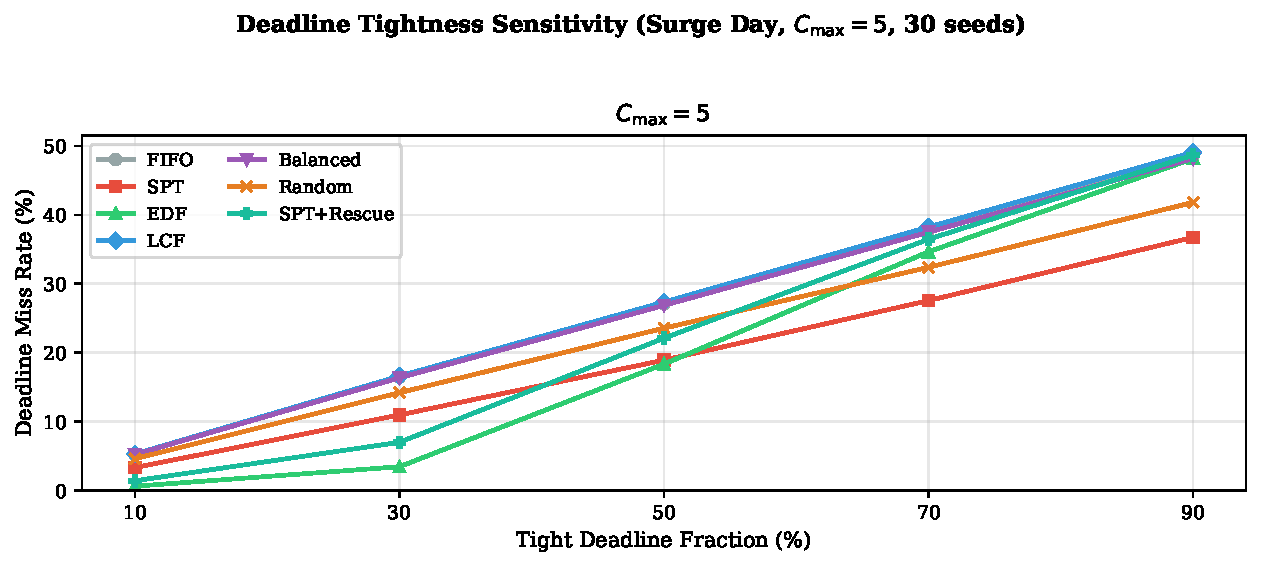
\includegraphics[width=0.98\linewidth,height=0.72\textheight,keepaspectratio]{figures/deadline_sensitivity.pdf}
\caption[Deadline-tightness sensitivity]{Deadline miss rate (\%) vs tight-deadline fraction (surge day, $C_{\max}=5$, 730 jobs, 30 seeds). EDF's miss is significantly lower than SPT's at $f_{\text{tight}} \leq 30\%$ and SPT's is significantly lower at $f_{\text{tight}} \geq 70\%$, while at $f_{\text{tight}} = 50\%$ the paired test does not resolve their difference ($\DlFiftySPTEDFmissP$), so the curves cross over an interval rather than at a point.}
\label{fig:deadline}
\end{figure}
\end{landscape}

No scheduler achieves 0\% miss across all tight-deadline fractions at surge-day load: although execution demand is below saturation, provisioning delays hold each slot and push waits to roughly \SensSrgWaitLo{} to \SensSrgWaitHi{}~min against 1\,h tight deadlines, so tight-deadline misses grow with $f_{\text{tight}}$ and are not removed by any ordering policy tested. Among the seven baseline policies in this sweep (RH, CADR, and Adaptive are not part of it), the EDF-SPT ordering reverses across the sweep, and a paired test at each of the five points locates the reversal rather than leaving it to the point estimates. The test is signed SPT minus EDF, so a positive $t$ favours EDF. EDF's miss is significantly lower at $f_{\text{tight}} = 10\%$ ($t=\DlTenSPTEDFmissT$, $\DlTenSPTEDFmissP$; \DlTenEDFmiss\% vs \DlTenSPTmiss\%) and at $f_{\text{tight}} = 30\%$ ($t=\DlThirtySPTEDFmissT$, $\DlThirtySPTEDFmissP$; \DlThirtyEDFmiss\% vs \DlThirtySPTmiss\%), with SPT+Rescue second-best at both. At $f_{\text{tight}} = 50\%$ the paired test does not resolve their difference ($t=\DlFiftySPTEDFmissT$, $\DlFiftySPTEDFmissP$): EDF's \DlFiftyEDFmiss\% and SPT's \DlFiftySPTmiss\% differ by less than the seed-to-seed variation, so the study names no winner at this point. SPT's miss is then significantly lower at $f_{\text{tight}} = 70\%$ ($t=\DlSeventySPTEDFmissT$, $\DlSeventySPTEDFmissP$; \DlSeventySPTmiss\% vs \DlSeventyEDFmiss\%) and at $f_{\text{tight}} = 90\%$ ($t=\DlNinetySPTEDFmissT$, $\DlNinetySPTEDFmissP$; \DlNinetySPTmiss\% vs \DlNinetyEDFmiss\%), where shortest-job-first ordering completes more jobs before their deadlines expire than deadline ordering does. The operational recommendation follows directly: use EDF or SPT+Rescue when the tight-deadline fraction is low ($f_{\text{tight}} \leq 30\%$) and switch to SPT once most jobs carry tight deadlines ($f_{\text{tight}} \geq 70\%$), with either choice defensible at $f_{\text{tight}} = 50\%$, where the paired test does not resolve their difference.

\subsection{Concurrency Limit Sensitivity}
\label{ssec:concurrency-limit-sensitivity}

The experiments fix $C_{\max}=5$, RunPod's default per-account worker quota; RunPod raises that quota in account-balance tiers (10 workers at \$100, up to 60 at \$900) or on request~\cite{runpod2026maxworkers}, and an operator may also cap concurrency below it for cost control. Table~\ref{tab:cmax_sensitivity} evaluates hectic-day performance ($n=10$ seeds, $\sim$950 jobs/day) across $C_{\max} \in \{3, 5, 7, 10\}$ to show how scheduler rankings shift under alternative provider policies; budgets above five are simulated what-ifs, since the calibration data never exceed five concurrent jobs. Figure~\ref{fig:cmax-sensitivity} plots the resulting saturation curves.

\begin{table}[htbp]
\centering
\caption[Concurrency limit sensitivity]{Concurrency limit sensitivity: avg wait (min) / miss\% on hectic day ($n=10$ seeds, $\sim$950 jobs/day, 20\% tight 1h / 80\% loose 8h deadlines); the $C_{\max}=5$ column therefore differs slightly from the 30-seed Phase~3 means. The \textbf{baseline} column ($C_{\max}=5$) is RunPod's default worker quota; the other columns correspond to tighter operator caps or higher RunPod quota tiers.}
\label{tab:cmax_sensitivity}
\begin{tabular}{lcccc}
\toprule
& \multicolumn{4}{c}{\textbf{Avg Wait (min) / Miss \%}} \\
\cmidrule(lr){2-5}
\textbf{Scheduler} & $C_{\max}=3$ & \shortstack{$C_{\max}=5$ \\ \textbf{(baseline)}} & $C_{\max}=7$ & $C_{\max}=10$ \\
\midrule
FIFO & 387.1\,/\,57.3 & 165.8\,/\,23.7 & 44.7\,/\,6.3 & 8.5\,/\,0.0 \\
SPT & 358.6\,/\,51.6 & 137.6\,/\,17.7 & 38.7\,/\,2.8 & 8.1\,/\,0.0 \\
EDF & 394.4\,/\,51.6 & 168.4\,/\,12.7 & 44.6\,/\,0.0 & 9.0\,/\,0.0 \\
SPT+Rescue & 372.1\,/\,49.7 & 144.7\,/\,13.5 & 39.0\,/\,0.0 & 8.1\,/\,0.0 \\
RH & 364.9\,/\,46.3 & 139.5\,/\,8.5 & 38.5\,/\,2.0 & 13.1\,/\,0.0 \\
CADR & 375.3\,/\,48.4 & 142.8\,/\,9.3 & 38.8\,/\,0.0 & 7.4\,/\,0.0 \\
Adaptive & 395.6\,/\,50.5 & 166.3\,/\,11.5 & 44.1\,/\,0.0 & 8.7\,/\,0.0 \\
\bottomrule
\end{tabular}

\end{table}

\begin{landscape}
\begin{figure}[H]
\centering
\captionsetup{font=small,skip=6pt}
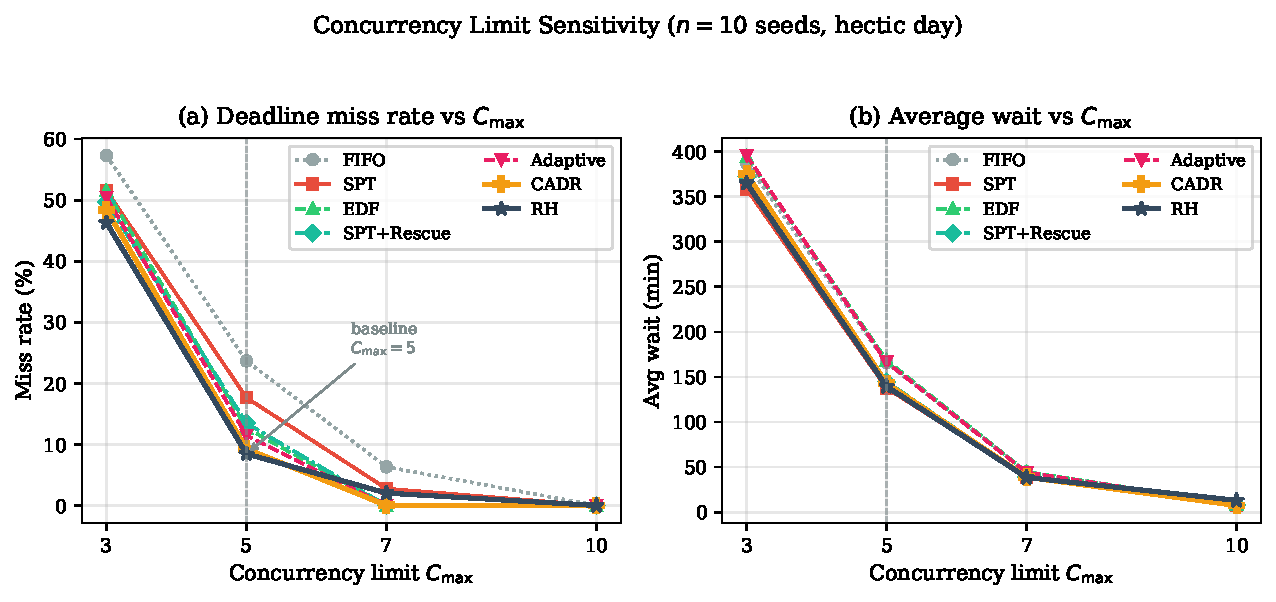
\includegraphics[width=0.98\linewidth,height=0.72\textheight,keepaspectratio]{figures/cmax_sensitivity.pdf}
\caption[Concurrency limit sensitivity]{Concurrency limit sensitivity: miss rate (a) and average wait (b) vs $C_{\max} \in \{3, 5, 7, 10\}$, $n=10$ seeds, hectic day. The dashed vertical line marks the $C_{\max}=5$ baseline. The saturation curve is clearly visible: the largest improvement in miss rate occurs between $C_{\max}=3$ and $C_{\max}=5$; gains are smaller from 5 to 7 and small from 7 to 10, where RH clears its remaining residual and FIFO its remaining \CmaxSevenFIFOmiss\%. At $C_{\max}=7$ the deadline-aware schedulers EDF, SPT+Rescue, CADR, and Adaptive reach near-zero miss (RH retains a small residual), but FIFO still lags at \CmaxSevenFIFOmiss\%, confirming that scheduler choice remains important even with more concurrency. The anomalous rise in RH's markedly higher wait at $C_{\max}=10$ (\CmaxTenRHwait{} against \CmaxTenOtherWaitLo{} to \CmaxTenOtherWaitHi{}~min for the other policies) relative to the other deadline-aware policies reflects the reservation mechanism briefly idling slots under the now-unsaturated load.}
\label{fig:cmax-sensitivity}
\end{figure}
\end{landscape}

At $C_{\max}=3$ (a restrictive provider policy) all schedulers incur high miss rates: with only three concurrent slots for $\sim$950 jobs/day ($\rho \gg 1$), the queue never drains, and even deadline-aware schedulers cannot prevent structural saturation misses. Under such a policy the choice of scheduling algorithm matters less than the concurrency ceiling itself. $C_{\max}=5$ (RunPod's default quota) is the binding operational constraint at hectic-day load: even the best deadline-aware schedulers still miss a substantial fraction of deadlines, whereas raising the budget by two slots to $C_{\max}=7$ brings deadline-aware schedulers to near-zero miss. At $C_{\max}=10$ every scheduler, FIFO included, reaches zero miss on the hectic day; mean waits are then about \CmaxTenOtherWaitLo{} to \CmaxTenOtherWaitHi~min for every policy except RH (\CmaxTenRHwait~min), whose reservation mechanism briefly idles slots under the unsaturated load. The scheduler comparison on miss is therefore decided at the baseline budget and below, and a budget large enough to clear a hectic day needs no scheduler help; the schedulers matter when the budget binds, as it does at the default quota of 5. The returns to added concurrency are diminishing: the miss reduction from $C_{\max}=3$ to $5$ is the largest single step, that from $5$ to $7$ is smaller, and from $7$ to $10$ smaller still. At $C_{\max}=7$ the deadline-aware policies drain the queue fast enough to meet almost every deadline, but FIFO continues to incur clearly elevated miss due to the absence of deadline ordering; only at $C_{\max}=10$ does FIFO also reach zero. This finding is practically relevant: if an operator's concurrency budget were raised to 7, an operator using FIFO would still benefit substantially from switching to a deadline-aware scheduler. Scheduler differences are largest at $C_{\max}=5$: at $C_{\max}=3$ all schedulers converge to near-total saturation, while at $C_{\max} \geq 7$ the deadline-aware schedulers converge to near-zero miss. The default $C_{\max}=5$ baseline therefore maximises the discriminating power of the scheduler comparison, because it is the point where the concurrency budget binds, and it provides the strongest motivation for deploying RH or CADR whenever the budget binds.

\subsection{Rescue Threshold Sensitivity}
\label{ssec:rescue-threshold-sensitivity}

Table~\ref{tab:threshold_sensitivity} sweeps the SPT+Rescue laxity threshold $\theta \in \{60, 180, 300, 600, 1200\}$\,s on hectic-day workload ($n=10$ seeds, $C_{\max}=5$, $\sim$950 jobs/day); Figure~\ref{fig:threshold-sensitivity} plots the sweep. The threshold controls when a job transitions from the normal SPT tier to the urgent EDF tier.

\begin{table}[htbp]
\centering
\caption[SPT+Rescue threshold sensitivity]{SPT+Rescue threshold sensitivity: avg wait (min) and miss\% on hectic day ($n=10$ seeds, $C_{\max}=5$, 20\% tight 1h / 80\% loose 8h deadlines). Minimum miss rate row is \textbf{bold}.}
\label{tab:threshold_sensitivity}
\begin{tabular}{lrr}
\toprule
\textbf{Threshold $\theta$} & \textbf{Avg Wait (min)} & \textbf{Miss \%} \\
\midrule
$\theta=60$\,s & 142.59 & 15.19 \\
$\theta=180$\,s & 142.04 & 11.66 \\
$\theta=300$\,s & 141.82 & 12.01 \\
\textbf{$\theta=600$\,s} (default) & 144.71 & 13.47 \\
$\theta=1200$\,s & 140.51 & \textbf{11.35} \\
\bottomrule
\end{tabular}

\end{table}



\Needspace{5\baselineskip}
Very small $\theta$ ($\leq 60$\,s) degrades SPT+Rescue towards plain-SPT behaviour: with a 60\,s threshold, few jobs enter the rescue tier early enough to be saved, so the mechanism yields the least benefit and the highest miss rate in the sweep (\ThrSixtyMiss\%). Beyond that, miss rate depends weakly and non-monotonically on $\theta$, varying within a narrow band. Across the whole sweep the miss rate stays within a \ThrMissSpread\,percentage-point band: it is highest at $\theta=60$\,s (\ThrSixtyMiss\%), reaches its lowest value at $\theta=180$\,s (\ThrOneEightyMiss\%), and is non-monotonic thereafter (\ThrSixHundredMiss\% at $\theta=600$\,s, \ThrTwelveHundredMiss\% at $\theta=1200$\,s). Mean wait varies only modestly over the sweep (a spread of roughly eight minutes) with no systematic trend in $\theta$. The mechanism is thus not sensitive to the exact threshold within a broad band, because the loose-deadline majority retains ample slack to absorb the reordering, and at $n=10$ the within-band differences are comparable to the sampling noise. It follows that $\theta = 600$\,s is an acceptable default. It is not the miss-minimising value in this $n=10$ sweep (the minimum is \ThrOneEightyMiss\% at $\theta=180$\,s), but because the miss rate varies by only \ThrMissSpread\,percentage points across the entire swept range, the choice of $\theta$ within this band is small relative to the $n=10$ seed noise. The default $\theta=600$\,s keeps mean wait moderate (\ThrSixHundredWait~min) and requires no fine tuning; a tighter $\theta$ around $180$\,s would lower the miss rate by \ThrDefaultGap\,percentage points, a gap that at $n=10$ lies within the noise band and is not separately optimised here (Table~\ref{tab:threshold_sensitivity}).


\begin{landscape}
\begin{figure}[H]
\centering
\captionsetup{font=small,skip=6pt}
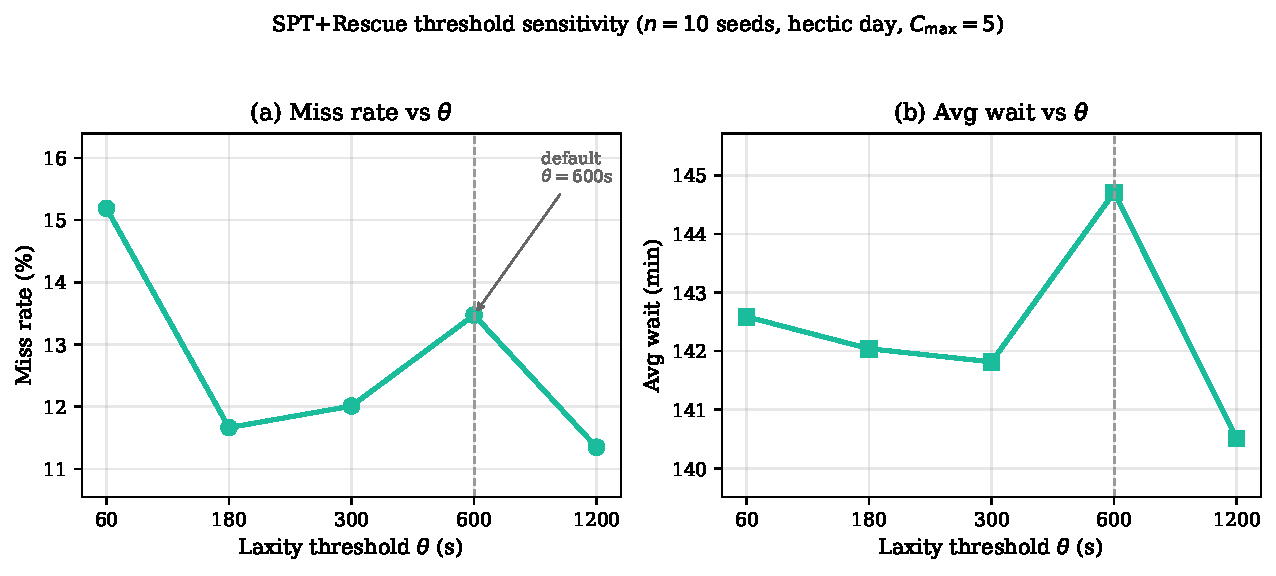
\includegraphics[width=0.98\linewidth,height=0.72\textheight,keepaspectratio]{figures/threshold_sensitivity.pdf}
\caption[SPT+Rescue threshold sensitivity]{SPT+Rescue laxity threshold $\theta$ sensitivity: miss rate (a) and average wait (b) across $\theta \in \{60, 180, 300, 600, 1200\}$\,s. The non-monotone shape of the miss rate curve is directly visible: the minimum is at $\theta=180$\,s; the curve then rises to its second-highest value at $\theta=300$\,s (\ThrThreeHundredMiss\%), dips at the default $\theta=600$\,s (\ThrSixHundredMiss\%), and rises slightly again at $\theta=1200$\,s (\ThrTwelveHundredMiss\%). The total variation across the whole range is \ThrMissSpread\,percentage points, confirming that the mechanism is robust to threshold choice within a broad interval. The dashed line marks the default $\theta=600$\,s.}
\label{fig:threshold-sensitivity}
\end{figure}
\end{landscape}

\subsection{Critical-Ratio Threshold Sensitivity}
\label{ssec:critical-ratio-threshold-sensitivity}

Table~\ref{tab:cr_sensitivity} sweeps the CADR critical-ratio threshold $\mathrm{CR}^*$ on hectic-day workload ($n=10$ seeds, $C_{\max}=5$, $\sim$950 jobs/day); Figure~\ref{fig:cr-sensitivity} plots the sweep. The threshold determines the boundary between the at-risk tier (dispatched EDF) and the safe tier (dispatched SPT); a higher $\mathrm{CR}^*$ promotes more jobs to the at-risk tier.

\begin{table}[htbp]
\centering
\caption[CADR critical-ratio threshold sensitivity]{Critical-ratio threshold sensitivity for CADR: avg wait (min) and miss\% on hectic day ($n=10$ seeds, $C_{\max}=5$). Minimum miss rate row is \textbf{bold}.}
\label{tab:cr_sensitivity}
\begin{tabular}{lrr}
\toprule
\textbf{$CR^{*}$ threshold} & \textbf{Avg Wait (min)} & \textbf{Miss \%} \\
\midrule
$CR^{*}=1.5$ & 142.94 & 11.47 \\
$CR^{*}=2.0$ & 142.34 & 10.14 \\
$CR^{*}=3.0$ & 142.80 & \textbf{9.28} \\
$CR^{*}=5.0$ & 143.94 & 9.96 \\
$CR^{*}=10.0$ & 145.10 & 10.05 \\
\bottomrule
\end{tabular}

\end{table}



\textbf{Critical-ratio sensitivity findings:} the CADR miss rate across the swept $\mathrm{CR}^*$ range has a best value of \CRStarBestMiss\% and a spread of only \CRStarMissSpread\,percentage points, confirming that the threshold is robust. The shipped default $\mathrm{CR}^*=\CRStarBestCR$ is itself the miss-minimising point of the sweep (\CRStarDefaultMiss\%, a gap of \CRStarDefaultGap\,pp to the sweep best), so it requires no tuning in practice; the miss rate is flat for $\mathrm{CR}^*\ge 3$ and rises at $\mathrm{CR}^*\le 2$ (CADR's lead over SPT+Rescue narrows at $\mathrm{CR}^*=2$ and is gone at $\mathrm{CR}^*=1.5$), so the default sits at the edge of the flat region rather than inside a wide plateau.


\begin{landscape}
\begin{figure}[H]
\centering
\captionsetup{font=small,skip=6pt}
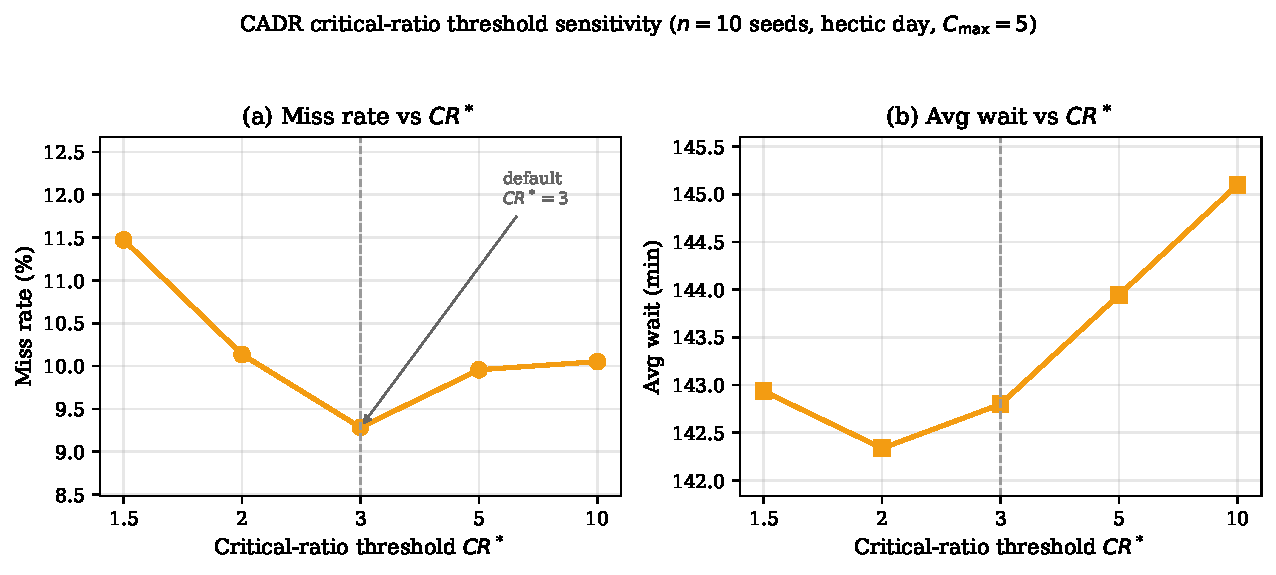
\includegraphics[width=0.98\linewidth,height=0.72\textheight,keepaspectratio]{figures/cr_sensitivity.pdf}
\caption[CADR critical-ratio threshold sensitivity]{CADR critical-ratio threshold $\mathrm{CR}^*$ sensitivity: miss rate (a) and average wait (b) across $\mathrm{CR}^* \in \{1.5, 2.0, 3.0, 5.0, 10.0\}$. The miss rate reaches its lowest value at $\mathrm{CR}^*=\CRStarBestCR$ (\CRStarBestMiss\%), which is the shipped default; the neighbouring $\mathrm{CR}^*=5$ sits a negligible fraction of a percentage point higher, well within the $n=10$ sampling noise, and the curve rises noticeably only at the low end ($\mathrm{CR}^* \leq 2$); the high extreme ($\mathrm{CR}^*=10$) stays essentially flat. The total spread is \CRStarMissSpread\,percentage points, confirming robustness to the exact threshold. Average wait is nearly flat across the entire range (\CRStarWaitSpread{}~min total variation). The dashed line marks the default $\mathrm{CR}^*=3$.}
\label{fig:cr-sensitivity}
\end{figure}
\end{landscape}

\subsection{Queue-Pressure Threshold Sensitivity}
\label{ssec:queue-pressure-threshold-sensitivity}

The Adaptive hybrid's queue-pressure threshold $P$ (the queue length above which its critical tier widens to the full loose window, Section~\ref{ssec:adaptive-queue-pressure-edf-spt-hybrid}) is the one tier threshold in the scheduler family not covered by the preceding sweeps, and its baseline value $P=10$ was otherwise unswept. Using the same protocol as the rescue-threshold and critical-ratio sweeps (hectic day, $C_{\max}=5$, $n=10$ seeds), $P \in \{3, 5, 10, 20, 50\}$ yields miss rates from \PswpBestMiss\% (at $P=\PswpBestP$) to a maximum \PswpSpread~percentage points higher, with the baseline $P=10$ at \PswpBaseMiss\% near the low end of the band (second lowest of five): comparable sensitivity to the rescue and critical-ratio thresholds, with no setting changing Adaptive's position in the comparison. In particular, the sweep minimum is a post-hoc best-of-five selection, and even that setting remains significantly worse than RH on the same ten seeds (paired difference $\PswpVsRHdiff$ percentage points \emph{against} Adaptive, $t=\PswpVsRHt$, $\PswpVsRHp$), so no $P$ in the swept range closes the gap to the proposed schedulers; the comparison is paired on the same seeds, as every headline comparison in this chapter is. Adaptive's tardiness advantage does persist across the sweep (best \PswpBestTardVal~min at $P=\PswpBestTardP$). The sweep is reproducible via \texttt{CGRSP/phase3\_pressure\_sensitivity.py}.

\subsection{Anticipation Reservation Sensitivity}
\label{ssec:anticipation-reservation-sensitivity}
Table~\ref{tab:reservation_sensitivity} sweeps the Rolling-Horizon reservation count $\rho_{\mathrm{res}} \in \{0, 1, 2, 3\}$ on two day types ($n=30$ seeds, $C_{\max}=5$): the surge day ($\lambda=0.020$ j/s, offered load below saturation) and the hectic day ($\lambda=0.100$ j/s, above saturation). The sweep isolates the contribution of reserving idle capacity for anticipated tight-deadline arrivals and verifies that the offered-load gate switches anticipation off when no spare capacity exists. Tight- and loose-deadline miss are reported separately because anticipation targets the tight (rush-order) jobs; Figure~\ref{fig:reservation-sensitivity} plots the miss rates for both day types.
\begin{table}[htbp]
\centering
\caption[Anticipation reservation sensitivity]{Anticipation reservation sensitivity: wait, overall miss\%, and tight/loose miss\% for reservation counts $\rho_{\mathrm{res}}$ on the surge day (below saturation) and hectic day (above saturation), $n=30$ seeds, $C_{\max}=5$. The lowest miss in each day group is in bold.}
\label{tab:reservation_sensitivity}
\begin{tabular}{llrrrr}
\toprule
\textbf{Day} & \textbf{$\rho_{\mathrm{res}}$} & \textbf{Wait (min)} & \textbf{Miss \%} & \textbf{Tight \%} & \textbf{Loose \%} \\
\midrule
\multirow{4}{*}{Surge ($\rho<1$)} & 0 (none) & 96.9 & 6.42 & 32.0 & 0.0 \\
 & 1 & 108.8 & \textbf{1.33} & 6.6 & 0.0 \\
 & 2 & 130.7 & 2.20 & 6.4 & 1.2 \\
 & 3 & 167.8 & 5.65 & 6.1 & 5.5 \\
\midrule
\multirow{4}{*}{Hectic ($\rho>1$)} & 0 (none) & 141.7 & \textbf{9.60} & 31.4 & 4.2 \\
 & 1 & 141.7 & \textbf{9.60} & 31.4 & 4.2 \\
 & 2 & 141.7 & \textbf{9.60} & 31.4 & 4.2 \\
 & 3 & 141.7 & \textbf{9.60} & 31.4 & 4.2 \\
\bottomrule
\end{tabular}

\end{table}

\begin{landscape}
\begin{figure}[H]
\centering
\captionsetup{font=small,skip=6pt}
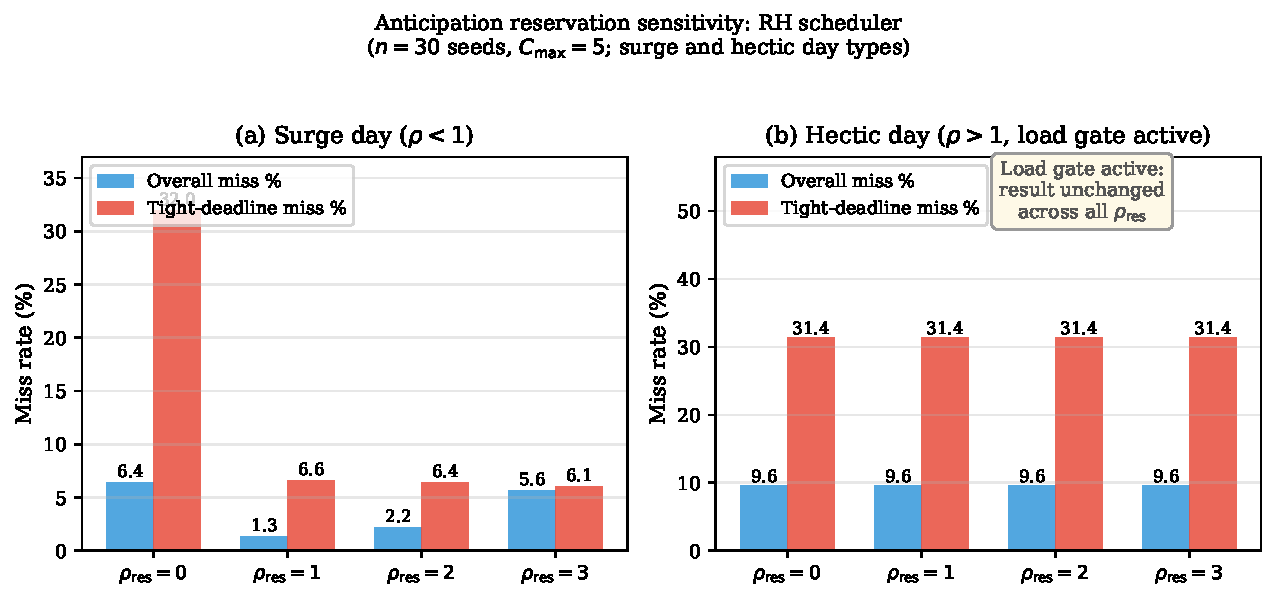
\includegraphics[width=0.98\linewidth,height=0.72\textheight,keepaspectratio]{figures/reservation_sensitivity.pdf}
\caption[Anticipation reservation sensitivity]{Anticipation reservation sensitivity for the RH scheduler: overall miss rate and tight-deadline miss rate for $\rho_{\mathrm{res}} \in \{0,1,2,3\}$ on the surge day (a, $\rho<1$) and the hectic day (b, $\rho>1$). On the surge day, a single reserved slot ($\rho_{\mathrm{res}}=1$) cuts tight-deadline miss from \ResSurgeOffTight\% to \ResSurgeOnTight\% at the cost of a modest wait increase. Reserving more slots ($\rho_{\mathrm{res}}=2,3$) offers diminishing returns and begins to push loose jobs into misses. On the hectic day, the load gate activates and all four $\rho_{\mathrm{res}}$ values produce identical results: reservation is disabled under saturation.}
\label{fig:reservation-sensitivity}
\end{figure}
\end{landscape}

\textbf{Reservation findings:} below saturation, anticipation yields a measurable benefit. On the surge day a single reserved slot ($\rho_{\mathrm{res}}=1$) cuts overall miss from \ResSurgeOffMiss\% to \ResSurgeOnMiss\% and tight-deadline miss from \ResSurgeOffTight\% to \ResSurgeOnTight\%, while loose-deadline miss stays negligible (\ResSurgeOnLoose\%): the eight-hour loose jobs have ample slack to absorb the brief idling, so their deadlines are unaffected, whereas the one-hour rush jobs that would otherwise be caught behind a burst now find a slot waiting. The cost is a modest rise in mean wait (\ResSurgeOffWait{} to \ResSurgeOnWait~min) from the deliberately idled capacity. Reserving more slots ($\rho_{\mathrm{res}}=2,3$) lowers tight miss slightly further but raises wait and begins to push loose jobs into misses, so a single reserved slot is the balanced operating point. On the hectic day every $\rho_{\mathrm{res}}$ produces the identical no-reservation result (\ResHecticGateMiss\% miss): the offered-load gate detects saturation and disables reservation, because withholding a slot from an already-saturated queue would only delay work that cannot be deferred. This load gating is why RH uses $\rho_{\mathrm{res}}=1$ throughout the study without disturbing the saturated-load headline results, which are produced with reservation gated off.


\subsection{Availability-Model Sensitivity}
\label{ssec:availability-model-sensitivity}

The per-type baseline high-stock probabilities $\beta_g$ are modelling assumptions for the on-demand pool (Section~\ref{ssec:platform-and-data}), so their influence on the scheduler comparison is tested directly: all four $\beta_g$ values are scaled by a common factor in $\{0.25, 0.50, 0.75, 1.00, 1.25\}$ and the hectic-day benchmark is re-run (30 seeds, six schedulers). Table~\ref{tab:beta_sensitivity} reports the outcome.

\begin{table}[htbp]
\centering
\caption[Availability-model sensitivity]{Availability-model ($\beta_g$) sensitivity on the hectic day ($C_{\max}=5$, 30 seeds). All four baseline high-stock probabilities are scaled by the factor in the first column; the baseline model is $\times 1.00$. Effective miss counts a job unfinished at the end of the 24-hour window as missed (every deadline in the instance falls before the window end), so the metric is immune to completion censoring at the extreme scales; the wait column, by contrast, is conditional on completion, which is why it is non-monotone across the two inoperable rows.}
\label{tab:beta_sensitivity}
\footnotesize
\setlength{\tabcolsep}{4pt}
\begin{tabular}{lrrrrrr}
\toprule
& \multicolumn{6}{c}{\textbf{Avg Wait (min) / Effective Miss \%}} \\
\cmidrule(lr){2-7}
\textbf{$\beta_g$ scale} & \textbf{FIFO} & \textbf{SPT} & \textbf{EDF} & \textbf{SPT+Rescue} & \textbf{RH} & \textbf{CADR} \\
\midrule
$\times0.25$ & 742.0\,/\,95.5 & 711.5\,/\,99.0 & 689.4\,/\,99.0 & 696.2\,/\,99.1 & 708.6\,/\,95.8 & 711.1\,/\,96.2 \\
$\times0.50$ & 906.8\,/\,91.3 & 894.1\,/\,93.3 & 907.2\,/\,97.3 & 905.6\,/\,97.5 & 900.1\,/\,89.6 & 903.2\,/\,91.6 \\
$\times0.75$ & 373.9\,/\,57.0 & 344.8\,/\,50.6 & 376.5\,/\,50.8 & 359.9\,/\,49.2 & 350.4\,/\,44.3 & 359.0\,/\,48.4 \\
$\times1.00$ \textbf{(baseline)} & 167.9\,/\,24.4 & 141.4\,/\,19.0 & 170.2\,/\,14.7 & 146.3\,/\,13.6 & 141.7\,/\,9.6 & 144.7\,/\,9.7 \\
$\times1.25$ & 87.5\,/\,12.3 & 75.6\,/\,6.4 & 86.8\,/\,0.0 & 76.7\,/\,0.0 & 75.4\,/\,5.4 & 76.9\,/\,0.0 \\
\bottomrule
\end{tabular}

\normalsize
\end{table}

Three regimes emerge, and the baseline row reproduces the Phase~3 means exactly, an incidental cross-check of the pipeline's determinism. First, availability is a first-order \emph{system} factor: at $\times 0.75$ every policy degrades steeply (effective miss \BetaThreeQuarterMinEffMiss\% to \BetaThreeQuarterMaxEffMiss\% across the full ten-policy grid, the upper end held by the deadline-blind LCF rather than by any policy in the table), and at $\times 0.50$ and below the Low state's 600 to 7{,}200\,s delays overwhelm the fleet outright: only \BetaHalfCompletedPct\% ($\times 0.50$) and \BetaQuarterCompletedPct\% ($\times 0.25$) of jobs finish within the day, and no policy, deadline-aware or not, gets its effective miss below \BetaHalfMinEffMiss\%. Second, and central to this thesis, the \emph{scheduler comparison} is stable on the scarcity side of the operable range: at $\times 0.75$ as at baseline, RH is lowest (\BetaThreeQRHmiss\%), CADR second (\BetaThreeQCADRmiss\%, closely followed by SPT+Rescue at \BetaThreeQRescueMiss\%), and the deadline-blind policies worst, so on the scarcity side the conclusions about scheduler ordering do not hinge on the exact calibration point. The ordering is statistically firm: paired $t$-tests on the published per-seed arrays at $\times 0.75$ give RH vs CADR $t=\BetaRHvCADRt$ ($\BetaRHvCADRp$) and RH vs SPT+Rescue $t=\BetaRHvRescueT$ ($\BetaRHvRescueP$). Third, at $\times 1.25$ the deadline problem becomes easy and the differences compress: CADR, EDF, and SPT+Rescue reach zero misses while RH retains a small residual (\BetaUpRHmiss\%, comparable to SPT's \BetaUpSPTmiss\%), so the RH advantage is a property of the baseline scarcity-and-saturation regime rather than a universal ordering. In summary, $\beta_g$ sets the system's overall difficulty, as expected for a per-dispatch delay term shared by all policies, while the relative merits of the schedulers, the object of this chapter, are stable across the scarcity side of the operable range ($\times 0.75$ to $\times 1.00$); on the eased side ($\times 1.25$), and under the data-ordered permutation below, the separation between deadline-aware and deadline-blind policies persists but RH yields the lead to CADR and SPT+Rescue. The sweep is reproducible via \texttt{CGRSP/phase3\_beta\_sensitivity.py}.

The remaining four policies (LCF, Balanced, Random, and the Adaptive hybrid) were also swept across all five scales (the full ten-policy grid is in the repository JSON): each tracks its Phase~3 cluster position at every operable scale, with the deadline-blind trio staying at the FIFO end and Adaptive staying adjacent to SPT+Rescue (swapping places with it at $\times 0.75$) and behind both proposed schedulers wherever the deadline problem is not already solved outright, so restricting the table to six policies discards no ordering information. Because a common scale factor perturbs the \emph{level} of the availability assumption but preserves its cross-type \emph{ranking}, two further checks target the ranking itself (both reproducible via \texttt{CGRSP/phase3\_prior\_robustness.py}). First, a data-ordered permutation: the four $\beta_g$ values are permuted so the RTX~3090 becomes the best-stocked type (0.75) and the RTX~A4000 the worst (0.50), which inverts the baseline ranking that the fixed per-type reliability priors in RH and Adaptive encode. This permutation is not a contrived stress case: it is the order in which the snapshot record ranks the four fleet types by the share of snapshots carrying any Secure Cloud offer (RTX~3090 94\%, RTX~A5000 86\%, RTX~A4500 72\%, RTX~A4000 63\%). That share measures whether a single-GPU listing is present rather than the probability that a request is fulfilled promptly, so it does not calibrate $\beta_g$, but it is the only per-type ranking the record offers, and it supports this permutation rather than the baseline ranking. Because the doubly-represented RTX~3090 inherits the highest availability, the fleet-weighted operating point becomes easier, and every policy improves: FIFO falls to \RevFIFOmiss\%, SPT to \RevSPTmiss\%, and the compressed easy-regime pattern of the $\times 1.25$ row reappears, with CADR (\RevCADRmiss\%) and SPT+Rescue (\RevRescueMiss\%) lowest, EDF (\RevEDFmiss\%) also ahead of RH, and RH at \RevRHmiss\% (significantly above CADR here, paired $t=\RevRHvCADRt$, $\RevRHvCADRp$). The deadline-blind anchor remains worst, one of the two proposed schedulers leads, and RH's own miss falls by roughly a third relative to its baseline, so the inverted prior degrades nothing catastrophically. The RH-versus-CADR order, however, does not survive: under the only per-type ranking the record supports, CADR leads and RH is significantly worse, so RH's miss lead over CADR at baseline is conditional on the assumed per-type scarcity ranking rather than robust to it, and that ranking is itself an assumption. Second, a direct ablation isolates the prior: RH re-run with the per-type reliability prior zeroed (stock-status penalty retained) on the baseline model gives \NoPriorRHmiss\% miss at \NoPriorRHwait~min wait, without a significant paired miss-rate difference from baseline RH (stock minus no-prior paired difference $\NoPriorDiffPp$ percentage points, $t=\NoPriorT$, $\NoPriorP$): this sample does not resolve a miss-rate effect from the fixed per-type prior, and does not establish that the prior is inert or that ordering alone explains RH's advantage. A third check in the same script targets the assumed arrival rate rather than $\beta_g$ (30 seeds; Section~\ref{ssec:anticipative-rolling-horizon-scheduler}): on the hectic day, assuming $0.5\times$ or $0.6\times$ the true rate (both below the gate's switching point of $\lambda\approx\PriorGateLambda$~jobs/s) lifts RH's miss from \RHMiss\% to \PriorHecUnderMiss\% and its wait from \RHWait{} to \PriorHecUnderWait~min, above FIFO's \FIFOwait~min, while every assumed rate from $0.75\times$ to $4\times$ reproduces the gated result exactly. On the surge day a $2\times$ over-estimate is inert and a $4\times$ one raises miss from \ResSurgeOnMiss\% to \ResSurgeOffMiss\%.

\subsection{Uncertainty in Estimated Execution Times}
\label{ssec:uncertainty-in-estimated-execution-times}

Three service-time cells have fewer than five observations and use estimated means and pooled log-space dispersion (Section~\ref{ssec:platform-and-data}). Their historical sample sizes do not measure their exposure in the synthetic workload: across six focal policies, these cells receive \SparseExposureLo\% to \SparseExposureHi\% of dispatches in the ten-seed baseline. Their uncertainty therefore warrants a direct check.

Table~\ref{tab:sparse_sensitivity} varies only those three cells: their means are scaled by $\times 0.75$ or $\times 1.25$, or their log-space dispersions by $\times 0.5$ or $\times 2$, while the dense cells, pricing and availability model are held fixed. These factors are modelling stress brackets, not confidence bounds estimated from the absent or sparse observations. Each arm runs the same ten seeds for FIFO, SPT, EDF, SPT+Rescue, RH and CADR; the baseline reproduces the first ten Phase~3 seeds, so it differs from the 30-seed headline. The load gate is recomputed from each arm's service model.

\begin{table}[htbp]
\centering
\caption[Estimated execution-cell sensitivity]{Deadline miss rate (\%) under estimated-cell mean and dispersion perturbations, hectic day, $C_{\max}=5$, ten paired seeds. Only the three cells with fewer than five observations are perturbed.}
\label{tab:sparse_sensitivity}
\small
\begin{tabular}{lrrrrrr}
\toprule
Estimated-cell arm & FIFO & SPT & EDF & SPT+Rescue & RH & CADR \\
\midrule
Baseline & 23.67 & 17.65 & 12.68 & 13.47 & 8.46 & 9.28 \\
Mean $\times 0.75$ & 20.76 & 12.16 & 8.40 & 6.17 & 7.07 & 5.17 \\
Mean $\times 1.25$ & 26.87 & 20.58 & 16.66 & 15.14 & 10.44 & 10.80 \\
$\sigma_{\ln}\times 0.5$ & 23.73 & 17.09 & 13.73 & 12.19 & 9.56 & 10.05 \\
$\sigma_{\ln}\times 2$ & 24.19 & 18.27 & 12.63 & 10.11 & 8.86 & 7.71 \\
\bottomrule
\end{tabular}

\end{table}

The numerical miss rates depend on these estimates. With lower estimated means, CADR has a lower point estimate than RH (\SparseMeanLowCADRMiss\% versus \SparseMeanLowRHMiss\%); with higher estimated means, RH has the lower point estimate (\SparseMeanHighRHMiss\% versus \SparseMeanHighCADRMiss\%). Neither mean perturbation separates the pair on an uncorrected paired test at 0.05. Halving the estimated-cell dispersion keeps RH ahead (\SparseSigmaLowRHMiss\% versus CADR's \SparseSigmaLowCADRMiss\%), whereas doubling it gives CADR the lower point estimate (\SparseSigmaHighCADRMiss\% versus RH's \SparseSigmaHighRHMiss\%); the raw paired $p=\SparseSigmaHighP$ for the doubled arm is not significant even before correction. The leading pair remains below the deadline-blind FIFO anchor in each tested arm, but the relative ordering and absolute miss rates should not be treated as insensitive to sparse calibration. The experiment is reproducible via \texttt{CGRSP/phase3\_sparse\_sensitivity.py}.

\subsection{Label Noise and GPU Speed Assumptions}
\label{ssec:label-noise-and-gpu-speed-assumptions}

Two assumptions in the calibration cannot be ruled out by the data and were previously only disclosed, not tested. First, the complexity class $\kappa$ is an ex-post render-time tercile that the model treats as known at arrival (Section~\ref{ssec:platform-and-data}); a deployed classifier would be imperfect. Second, the A4000 stratum means are not scene-matched: after the concurrency exclusion only two scenes are rendered on both the A4000 and the A5000, and on them its geometric-mean render time is 1.165 times the A5000's (an indicative value from very few scenes), while its pooled $\kappa=3$ stratum mean is 4\% above the A5000's (98.6\,s against 94.5\,s).

Table~\ref{tab:kappa_speed_sensitivity} brackets both on the hectic day ($C_{\max}=5$, ten seeds; the Baseline row is the ten-seed hectic-day result, as in Table~\ref{tab:sparse_sensitivity}, not the 30-seed Phase~3 figure). In the label arms the schedulers plan with an observed class that differs from the realised one; execution times, and therefore completion times and costs, always use the true class. ``Label error'' moves a job to an adjacent class with the stated probability (Low and High move to Medium, Medium moves to Low or High with equal probability); ``uninformative'' draws the observed class from the class mix independently of the job. In the speed arm every A4000 cell is scaled so that $\overline{W}(3,\text{A4000})=1.165\,\overline{W}(3,\text{A5000})$. These are stress brackets, not estimates: no classifier accuracy or corrected speed has been measured.

\begin{table}[htbp]
\centering
\caption[Complexity-label and A4000 speed sensitivity]{Deadline miss rate (\%) under complexity-label noise and a scene-matched A4000 speed, hectic day, $C_{\max}=5$, ten paired seeds. FIFO ignores the label.}
\label{tab:kappa_speed_sensitivity}
\small
\begin{tabular}{lrrrrrr}
\toprule
Arm & FIFO & SPT & EDF & SPT+Rescue & RH & CADR \\
\midrule
Baseline & 23.67 & 17.65 & 12.68 & 13.47 & 8.46 & 9.28 \\
Label error 20\% & 23.67 & 19.55 & 14.19 & 13.55 & 9.65 & 10.02 \\
Label error 40\% & 23.67 & 20.66 & 13.67 & 15.52 & 10.51 & 11.82 \\
Uninformative label & 23.67 & 23.96 & 13.07 & 18.22 & 13.02 & 14.24 \\
A4000 $\times 1.165$ & 25.92 & 20.76 & 16.76 & 14.56 & 9.28 & 11.25 \\
\bottomrule
\end{tabular}

\end{table}

RH has the lowest miss point estimate in every arm and stays below FIFO, and CADR is second in every arm except the uninformative one, where EDF (\KsUninfEDFMiss\%) is second (point estimates only: only the RH-versus-CADR pair is tested, so their separation from EDF and SPT+Rescue is not). Both have a higher miss point estimate in every degraded-label arm than at baseline (the rise reaches a raw paired-test $p<0.05$ only under the uninformative label, for RH, CADR, SPT and SPT+Rescue, and at 40\% label error for SPT and SPT+Rescue, and the rises are not monotone in the noise level; EDF, which uses the label only for node choice, also rises but not significantly in any label arm): with an uninformative label RH rises from \KsBaseRHMiss\% to \KsUninfRHMiss\% and CADR from \KsBaseCADRMiss\% to \KsUninfCADRMiss\%, leaving RH level with EDF and CADR about one point above it. The label matters most to the policies that rank jobs by estimated duration: SPT's point estimate (\KsUninfSPTMiss\%) is then above FIFO's (\KsUninfFIFOMiss\%), so its advantage over FIFO depends on the class being informative. RH has the lower point estimate than CADR in every arm, but only the scene-matched A4000 arm separates the pair on an uncorrected paired test at 0.05 (raw $p=\KsSlowRHvCADRp$, RH lower), and that arm rests on a ratio measured on only two scenes. The scene-matched A4000 raises every policy's miss rate (FIFO \KsSlowFIFOMiss\%, RH \KsSlowRHMiss\%, CADR \KsSlowCADRMiss\%; the rise is significant at raw 0.05 for FIFO, SPT and EDF) because scaling every A4000 cell by about 1.12 cuts the fleet's effective capacity at a load that already saturates it; no separate mechanism arm was run. The top of the ranking therefore holds at the level of point estimates, but the absolute miss rates in the main results are conditional on an oracle label and on the pooled A4000 mean. The experiment is reproducible via \texttt{CGRSP/phase3\_kappa\_speed\_sensitivity.py}.

\subsection{Objective-Weight Sensitivity}
\label{ssec:objective-weight-sensitivity}

The primary objective (Section~\ref{sec:mathematical-model}) is lexicographic: quality of service first, operational cost only as a tiebreaker among QoS-equivalent options. This section stress-tests that modelling choice by instead re-scoring the six focal schedulers under a fully symmetric weighted-sum scalarisation that treats QoS and cost as co-equal, $w_{\text{qos}}\, C_{\text{QoS}} + w_{\text{cost}}\, C_{\text{Cost}}$, across a grid of weights. The purpose is to show what the lexicographic priority deliberately avoids: that a symmetric scalar can be swayed by a cost difference that is near-noise at this fleet scale. Eight of the ten schedulers apply a fixed structural rule (shortest-job-first, earliest-deadline-first, laxity rescue, queue-pressure tiering, and so on) that never references the swept weights, so their decomposed metrics (wait, miss, cost) are \emph{by construction} independent of the weight choice. The Rolling-Horizon and CADR schedulers do reference cost during dispatch, but only as a minor term subordinate to the QoS penalty (RH) or as a tiebreaker among deadline-feasible nodes (CADR), and their decisions are held at that fixed configuration rather than re-optimised at each grid point.

For each of six focal schedulers (FIFO, SPT, EDF, SPT+Rescue, RH and CADR), per-seed waiting time, deadline-miss rate, and operational cost are collected on the hectic-day workload ($n=10$ seeds) and the composite objective is then evaluated post-hoc across a grid of weights. The mean per-job QoS penalty is $\alpha_1(60\,\overline{w}_{\rm min}) + \alpha_2(\Delta_{\rm miss,\%}/100)$, so wait is converted to seconds and miss percentage to a fraction before weighting. Thus $\alpha_2/\alpha_1=10$ equates one missed job with ten seconds of waiting, not with ten minutes or ten percentage points. Because the raw QoS component (seconds) and cost component (US dollars) lie on very different scales, each component is min-max normalised across the six focal schedulers before the weights are applied, so that $w_{\text{cost}}$ has a genuine effect on the ranking (a raw weighted sum would be entirely QoS-dominated). Table~\ref{tab:weight_sensitivity} reports two sweeps: the multi-objective weight $w_{\text{cost}} \in \{0.1, 0.3, 0.5, 0.7, 0.9\}$ (with the QoS ratio fixed at the baseline $\alpha_2/\alpha_1 = 10$), and the deadline-penalty ratio $\alpha_2/\alpha_1 \in \{1, 5, 10, 20, 50\}$ (with $w_{\text{qos}} = w_{\text{cost}} = 0.5$); Figure~\ref{fig:weight-sensitivity} plots the deadline-penalty sweep for both the miss-indicator and the tardiness objective.

\begin{table}[htbp]
\centering
\caption[Objective-weight sensitivity]{Objective-weight sensitivity: normalised composite objective per scheduler (lower is better) on the hectic day ($n=10$ seeds, $C_{\max}=5$). Components are min-max normalised across schedulers before weighting. The minimum (winning) scheduler in each row is \textbf{bold}; the symmetric reference configuration ($w_{\text{qos}}=w_{\text{cost}}=0.5$, $\alpha_2/\alpha_1=10$) appears as the marked row in both panels.}
\label{tab:weight_sensitivity}
\begin{tabular}{lrrrrrr}
\toprule
& \multicolumn{6}{c}{\textbf{Composite objective (normalised, lower is better)}} \\
\cmidrule(lr){2-7}
\textbf{Weight setting} & \textbf{FIFO} & \textbf{SPT} & \textbf{EDF} & \textbf{SPT+Rescue} & \textbf{RH} & \textbf{CADR} \\
\midrule
$w_{\text{cost}}=0.1$ & 0.92 & \textbf{0.04} & 0.99 & 0.21 & 0.12 & 0.22 \\
$w_{\text{cost}}=0.3$ & 0.94 & \textbf{0.11} & 0.98 & 0.16 & 0.24 & 0.34 \\
$w_{\text{cost}}=0.5$ \textbf{(baseline)} & 0.96 & 0.18 & 0.96 & \textbf{0.12} & 0.36 & 0.45 \\
$w_{\text{cost}}=0.7$ & 0.97 & 0.25 & 0.95 & \textbf{0.07} & 0.48 & 0.57 \\
$w_{\text{cost}}=0.9$ & 0.99 & 0.32 & 0.93 & \textbf{0.02} & 0.61 & 0.68 \\
\midrule
$\alpha_2/\alpha_1=1$ & 0.96 & 0.18 & 0.96 & \textbf{0.12} & 0.36 & 0.45 \\
$\alpha_2/\alpha_1=5$ & 0.96 & 0.18 & 0.96 & \textbf{0.12} & 0.36 & 0.45 \\
$\alpha_2/\alpha_1=10$ \textbf{(baseline)} & 0.96 & 0.18 & 0.96 & \textbf{0.12} & 0.36 & 0.45 \\
$\alpha_2/\alpha_1=20$ & 0.96 & 0.18 & 0.96 & \textbf{0.11} & 0.36 & 0.45 \\
$\alpha_2/\alpha_1=50$ & 0.96 & 0.18 & 0.96 & \textbf{0.11} & 0.36 & 0.45 \\
\bottomrule
\end{tabular}

\end{table}

No scheduler wins every weighting on this grid. SPT wins at the two lowest cost weights ($w_{\text{cost}}=0.1$ and $0.3$), where the wait term dominates the composite, and SPT+Rescue wins from $w_{\text{cost}}=0.5$ upward and at every deadline-penalty ratio; RH never wins, placing second at $w_{\text{cost}}=0.1$ and third elsewhere, and CADR is fourth throughout. The ranking is decided by cost, not by QoS: on these ten seeds SPT+Rescue is the cheapest policy (\$6.34 against \$6.37 for RH, \$6.38 for CADR and \$6.39 for FIFO and EDF, a spread of 0.9\%), and min-max normalisation stretches that sub-one-percent spread over the whole 0 to 1 scale, so once $w_{\text{cost}}$ reaches 0.5 a cost gap of a few cents outweighs RH's lowest miss rate. EDF and FIFO have the highest composites throughout because they have the highest mean waits. The 30-seed Phase~3 cost ranking differs (SPT is cheapest there), so this ordering is itself a ten-seed point estimate.

Under the symmetric scalar, the winner changes with the cost weight and is decided by a cost difference of under one percent that lies within seed noise, so the scalarisation fragility that motivates a lexicographic rather than a symmetric objective is demonstrated here directly: a symmetric scalar can place a policy that misses substantially more deadlines (SPT+Rescue) above the miss leader (RH) because of a few cents of rental cost. The thesis therefore adopts the lexicographic form (Section~\ref{sec:mathematical-model}) as the principled choice, since the lexicographic priority rules such a reordering out by construction rather than leaving it to the weights.

The decomposed conclusions are unaffected. RH holds the lowest miss point estimate among the focal schedulers irrespective of the weights (the 30-seed Phase~3 means are \RHMiss\% and \RHWait~min; the ten-seed subset used here gives slightly lower values), and the composite win of SPT+Rescue on this grid does not contradict those decomposed metrics; it reflects the cost axis alone. This is why the primary comparisons in this thesis report wait, miss, and cost separately (Section~\ref{sec:mathematical-model}) rather than collapsing them into a single weighted score. Operational cost headroom is structurally small across all policies, and CADR's cost-aware node selection does not make it the cheapest policy overall; the cost differences across all schedulers are near-noise at this scale, which is exactly why they can decide a min-max normalised composite.

\textbf{Tardiness-objective robustness.} As an additional check, each scheduler is re-scored post-hoc against a tardiness-based objective (replacing the dimensionless binary miss indicator $1-\delta_j$ with continuous tardiness $\tau_j$ measured in seconds) on the same hectic-day workload ($n=10$ seeds). The same numerical $\alpha_2/\alpha_1$ grid is reused, but its units change: in the binary score the ratio is seconds of waiting per missed job, whereas in the tardiness score it is seconds of waiting per second of lateness. Thus the change in winner reflects both the penalty form and its effective scale, not a controlled comparison at equal economic penalty per breach. Table~\ref{tab:tardiness_objective} reports the resulting composite scores.

\begin{table}[htbp]
\centering
\caption[Tardiness-objective re-scoring]{Tardiness-objective re-scoring: normalised composite score with a tardiness term (lower is better) by deadline-penalty ratio, hectic day ($n=10$ seeds, $C_{\max}=5$). Compare with the miss-indicator objective in Table~\ref{tab:weight_sensitivity}.}
\label{tab:tardiness_objective}
{\small\begin{tabular}{lrrrrrr}
\toprule
& \multicolumn{6}{c}{\textbf{Composite with tardiness term (normalised, lower is better)}} \\
\cmidrule(lr){2-7}
\textbf{$\alpha_2/\alpha_1$} & \textbf{FIFO} & \textbf{SPT} & \textbf{EDF} & \textbf{SPT+Rescue} & \textbf{RH} & \textbf{CADR} \\
\midrule
$\alpha_2/\alpha_1=1$ & 1.00 & 0.18 & 0.75 & \textbf{0.03} & 0.59 & 0.37 \\
$\alpha_2/\alpha_1=5$ & 0.98 & 0.26 & 0.54 & \textbf{0.02} & 0.83 & 0.37 \\
$\alpha_2/\alpha_1=10$ & 0.93 & 0.27 & 0.49 & \textbf{0.01} & 0.83 & 0.37 \\
$\alpha_2/\alpha_1=20$ & 0.91 & 0.28 & 0.47 & \textbf{0.01} & 0.83 & 0.37 \\
$\alpha_2/\alpha_1=50$ & 0.89 & 0.29 & 0.46 & \textbf{0.02} & 0.83 & 0.38 \\
\bottomrule
\end{tabular}
}
\end{table}

\begin{landscape}
\begin{figure}[H]
\centering
\captionsetup{font=small,skip=6pt}
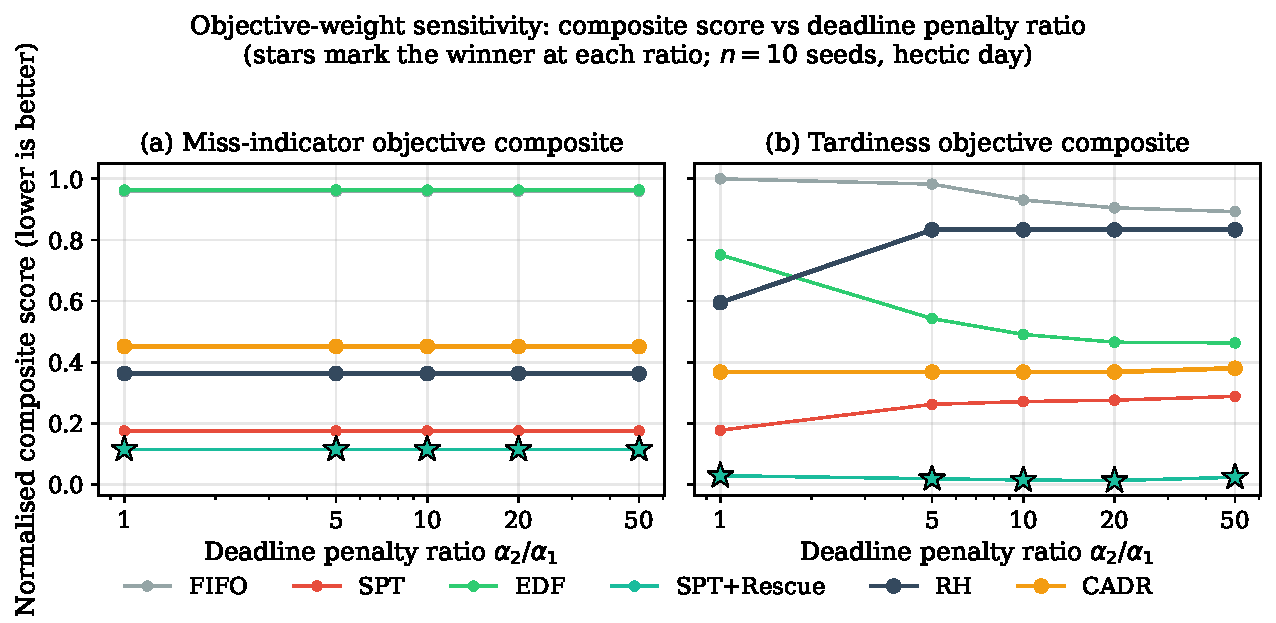
\includegraphics[width=0.98\linewidth,height=0.72\textheight,keepaspectratio]{figures/weight_sensitivity.pdf}
\caption[Objective-weight sensitivity]{Objective-weight sensitivity: normalised composite score (lower is better) versus the deadline-penalty ratio $\alpha_2/\alpha_1$ at the symmetric weighting $w_{\text{qos}}=w_{\text{cost}}=0.5$. Stars mark the winner at each ratio. Panel~(a), miss-indicator objective: SPT+Rescue wins at every ratio, reflecting its lowest cost on these ten seeds and a wait close to SPT's; the panel is essentially flat in the ratio (every composite moves by under 0.002 between $\alpha_2/\alpha_1=1$ and $50$) because the scaled wait term dominates the QoS score, so it tests the winner, not sensitivity to the ratio. Panel~(b), tardiness objective: SPT+Rescue also wins at every ratio; RH's score starts lower (third of the six at $\alpha_2/\alpha_1=1$) but rises sharply as the ratio grows, plateauing at a mid-pack value by $\alpha_2/\alpha_1=10$, because tight jobs it promotes too late fall into its demoted tier and carry high tardiness that is increasingly penalised as the ratio grows; EDF's score falls as the ratio grows since its low tardiness is increasingly rewarded, though it remains behind SPT+Rescue, SPT and CADR. The scalarised winner is the same in both scores here, while the per-metric leaders (Table~\ref{tab:statistical}) are different policies.}
\label{fig:weight-sensitivity}
\end{figure}
\end{landscape}

The tardiness composite is also won by SPT+Rescue at every penalty ratio (Table~\ref{tab:tardiness_objective}), followed by SPT and then CADR: SPT+Rescue combines the lowest cost on these ten seeds with a wait close to SPT's and a low mean tardiness, while CADR's lower tardiness is outweighed by its slightly higher wait and cost. RH, the miss-count leader on point estimate, drops to a lower-mid score here and does not improve as the tardiness weight $\alpha_2/\alpha_1$ rises, because RH's late promotion of tight jobs, which then fall into its demoted tier, gives it the highest mean tardiness of the six schedulers compared here (Random's tardiness is higher still in the full ten-scheduler comparison of Section~\ref{sec:phase-3-statistical-validation}); EDF's score falls as that weight grows, since its low tardiness is increasingly rewarded, though it remains behind SPT+Rescue, SPT and CADR throughout. This does not indicate a robustness failure; it sharpens the central distinction of the thesis: RH minimises the \emph{count} of missed deadlines, not their severity, so it does not lead a tardiness-weighted objective under any ratio tested. The per-metric leaders are RH for miss count and, among the two proposed schedulers, CADR for tardiness (Adaptive, EDF and SPT+Rescue post comparably low tardiness but do not match RH or CADR on miss); the single scalarised winner is a third policy, SPT+Rescue, whose edge comes from cost and wait, and the rescoring cannot attribute any change in winner solely to the penalty form, since its units and effective scale also differ. The practical reading is therefore objective-dependent by design: an operator who penalises lateness continuously should use CADR rather than RH, and since the paired baseline binary-miss test does not resolve the difference between them, CADR is also the default for an operator who penalises misses as binary events, with RH kept as the specialist for the scarce baseline regime, where its miss point estimate is lowest (Section~\ref{sec:mathematical-model}).

\subsection{Fleet-Composition Sensitivity}
\label{ssec:fleet-composition-sensitivity}

The headline fleet is fixed at two RTX~3090 slots and one each of the RTX~A5000, A4500 and A4000. Table~\ref{tab:fleet_mix} reports the mean miss rate for the six mixes. To test whether the policy ordering depends on that composition, six five-slot mixes are run for ten seeds (0 to 9) each: the all-types anchor, three mixes in which one type occupies three slots, and two single-type fleets. The anchor reproduces the first ten seeds of the Phase~3 record in \texttt{statistical.json} exactly (360 of 360 compared values across six policies and six metrics), so it is the same workload and dispatch path as the headline experiment. The other mixes keep the job stream and the policy implementations, but a different fleet changes which slot is free at each dispatch, so their service draws need not match the anchor seed by seed. The sweep is a sensitivity check at $n=10$, not a second workload, and it is not a second studio trace.

\begin{table}[htbp]
\centering
\caption[Fleet-composition sensitivity]{Fleet-composition sensitivity: mean deadline miss rate (\%) for six five-slot mixes, ten seeds each, on the Phase~3 hectic day ($\sim$950 jobs/day, $C_{\max}=5$, $\lambda=0.100$ j/s, 20\% tight 1h / 80\% loose 8h deadlines). The Slots column gives the slot counts in the order RTX~3090 / RTX~A5000 / RTX~A4500 / RTX~A4000. Bold marks the lowest miss rate in each row. The all-types row reproduces the first ten Phase~3 seeds; the other rows are sensitivity checks at $n=10$, not separate headline tests.}
\label{tab:fleet_mix}
\small
\begin{tabular}{llrrrrrr}
\toprule
\textbf{Mix} & \textbf{Slots} & \textbf{FIFO} & \textbf{SPT} & \textbf{EDF} & \textbf{SPT+Rescue} & \textbf{RH} & \textbf{CADR} \\
\midrule
All-types & 2/1/1/1 & 23.67 & 17.65 & 12.68 & 13.47 & \textbf{8.46} & 9.28 \\
3090-heavy & 3/1/0/1 & 28.51 & 22.01 & 18.14 & 17.37 & \textbf{12.94} & 13.46 \\
A5000-heavy & 1/3/0/1 & 23.60 & 16.77 & 12.79 & 9.13 & 9.27 & \textbf{8.15} \\
A4000-heavy & 1/1/0/3 & 15.79 & 7.31 & 2.07 & 1.36 & 5.96 & \textbf{0.57} \\
3090-only & 5/0/0/0 & 36.23 & 31.14 & 28.13 & 25.71 & \textbf{22.11} & 23.12 \\
A5000-only & 0/5/0/0 & 25.43 & 19.42 & 14.45 & 13.85 & \textbf{8.84} & 9.55 \\
\bottomrule
\end{tabular}

\end{table}

Two features are stable across the six mixes. First, RH and CADR are the two lowest-miss policies in the all-types, 3090-heavy, 3090-only and A5000-only mixes. Second, every deadline-aware policy (EDF, SPT+Rescue, RH and CADR) has a lower mean miss than FIFO in every mix. The ordering is not stable overall: the JSON's ordering flag is false because the A5000-heavy and A4000-heavy mixes place CADR and SPT+Rescue in the two lowest positions, with RH third and fourth respectively.

The A5000-heavy reversal is a point-estimate ordering, not a resolved one. RH and CADR differ by 1.12 percentage points (9.27\% against 8.15\%, paired $p=0.282$, pooled $d=0.287$), and RH and SPT+Rescue differ by 0.14 points ($p=0.916$, pooled $d=0.041$). Neither difference is significant, so this mix does not establish that either policy is better on miss; it shows only that RH's lead does not persist in the point estimates.

The A4000-heavy reversal is decisive. CADR's 0.57\% miss is far below RH's 5.96\% (paired $p<0.001$, pooled $d=6.21$), and SPT+Rescue (1.36\%) is also below RH (uncorrected $p=0.0038$). This is the easiest mix in the sweep for every policy, with FIFO at 15.79\% against 23.67\% in the anchor, but CADR's advantage over RH is significant and large.

Across the six mixes, RH is the lowest-miss point estimate in four and CADR in two. CADR is never more than about one percentage point above the mix minimum (its largest gap is 1.01 points in the 3090-only mix), whereas RH falls 5.39 points behind in the A4000-heavy mix. The ordering is therefore composition-dependent, and CADR is the more robust default: it is at or near the minimum in every mix and leads in the two mixes where RH's lead reverses. RH remains the lowest-miss policy in four of the six mixes, including the baseline all-types fleet; the composition dependence, not a universal RH lead, is the finding. The $n=10$ sweep is a sensitivity check, not a headline test, and the cross-mix service draws differ in dispatch order; a second studio trace remains the open generalisation test.

\section{Phase 4: Monthly Operational Simulation}
\label{sec:phase-4-monthly-operational-simulation}

Phases 2 and 3 benchmark schedulers on hectic-day workload ($\sim$950 jobs/day) and characterise performance across all day types. Phase 4 evaluates the same schedulers over a month whose day-type mix is taken from RunPod billing, with each day type's job count as in Section~\ref{ssec:platform-and-data}. Because every hectic day carries the assumed stress-load count, a simulated month holds about 7,600 jobs on average over the ten replications, roughly 60\% of them on hectic days. That is about three times the busiest month in the job record (about 2,400 jobs, September 2025). Phase~4 therefore spreads the hectic-day stress-load assumption over a billing-derived calendar rather than testing it independently.

\textbf{Results.} Table~\ref{tab:phase4} summarises monthly outcomes; Figure~\ref{fig:cost-comparison} isolates the cost dimension for both the hectic-day and the monthly horizon. Figure~\ref{fig:phase4} shows waiting time by day type and monthly deadline miss rates. Figure~\ref{fig:phase4-timeline} shows the daily miss rate trajectory over a representative 30-day replication, illustrating how performance tracks the day-type sequence: hectic and surge days produce sharp spikes while normal and quiet days remain near zero for all schedulers.

\begin{table}[htbp]
\centering
\caption[Phase 4 monthly summary]{Phase 4 monthly outcome summary per scheduler: wait, miss, tardiness, and cost ($C_{\max}=5$, 30 days, 10 replications, 20\% tight 1h / 80\% loose 8h deadlines)}
\label{tab:phase4}
\resizebox{\linewidth}{!}{\begin{tabular}{lrrrrr}
\toprule
\textbf{Scheduler} & \textbf{Avg Wait (min)} & \textbf{95\% CI} & \textbf{Miss\%} & \textbf{Avg Tardiness (min)} & \textbf{Cost (\$/mo)} \\
\midrule
\textbf{RH} & 103.73 & [95.28,~112.17] & \textbf{6.57} & 19.07 & 48.31 \\
CADR & 104.09 & [95.14,~113.03] & 7.06 & 6.27 & 48.43 \\
SPT+Rescue & 104.29 & [95.83,~112.75] & 8.96 & 5.19 & 48.67 \\
Adaptive & 116.81 & [107.85,~125.78] & 7.53 & 3.51 & 48.67 \\
\textbf{SPT} & \textbf{101.92} & [93.18,~110.66] & 12.86 & 10.69 & 48.56 \\
EDF & 116.69 & [106.50,~126.88] & 8.92 & 3.77 & 50.67 \\
LCF & 114.64 & [105.08,~124.20] & 16.50 & 17.82 & 48.52 \\
Balanced & 116.70 & [106.64,~126.77] & 16.55 & 18.26 & 49.11 \\
FIFO & 116.09 & [106.21,~125.97] & 16.74 & 18.02 & 53.08 \\
Random & 116.39 & [106.08,~126.71] & 15.62 & 22.32 & 51.48 \\
\bottomrule
\end{tabular}
}
\end{table}

\begin{landscape}
\begin{figure}[H]
\centering
\captionsetup{font=small,skip=6pt}
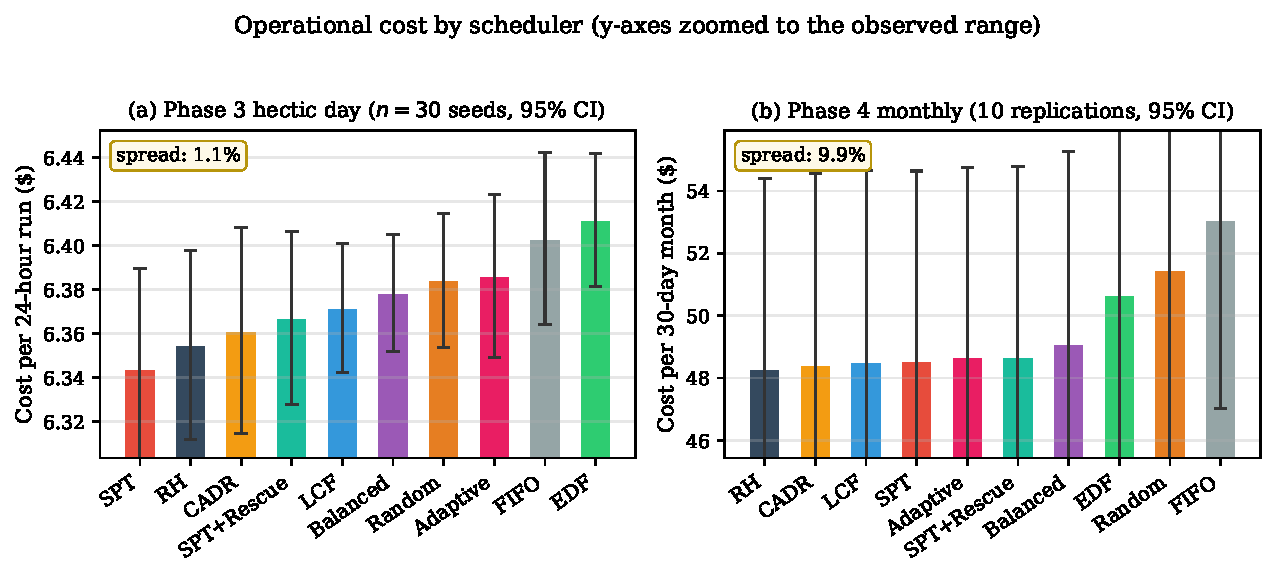
\includegraphics[width=0.98\linewidth,height=0.72\textheight,keepaspectratio]{figures/cost_comparison.pdf}
\caption[Operational cost by scheduler]{Operational cost by scheduler, with y-axes zoomed to the observed range and 95\% confidence intervals. (a)~Phase~3 hectic-day cost per 24-hour run: the spread between the cheapest and most expensive policy (SPT and EDF) is about \CostSpreadPct\%, small beside the QoS differences, and the confidence intervals of every pair of policies overlap, which is why cost cannot meaningfully discriminate between the schedulers under saturation. (b)~Phase~4 monthly cost across the full day-type mix: the spread widens (FIFO, Random, and EDF incur the highest monthly costs), but the confidence intervals still overlap heavily, and the two proposed schedulers sit at the cheap end of the range.}
\label{fig:cost-comparison}
\end{figure}
\end{landscape}

\begin{landscape}
\begin{figure}[H]
\centering
\captionsetup{font=small,skip=6pt}
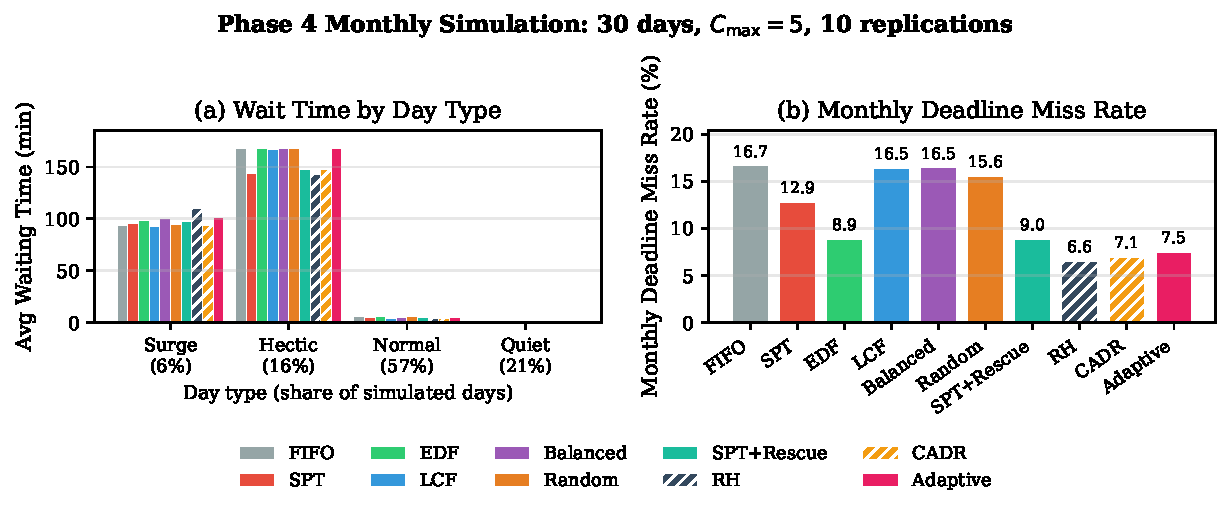
\includegraphics[width=0.98\linewidth,height=0.72\textheight,keepaspectratio]{figures/phase4_monthly.pdf}
\caption[Phase 4 monthly results]{Phase 4 monthly simulation ($C_{\max}=5$, 30 days, 10 replications, 20\% tight 1h / 80\% loose 8h). (a) Average waiting time by day type: the hectic cohorts have the largest wait, surge cohorts also show substantial queueing, and normal and quiet cohorts have much smaller waits. (b) Monthly miss rate: RH \PhFourRHMiss\% and CADR \PhFourCADRMiss\% (the lowest tier; no paired test is computed at this phase), SPT+Rescue \PhFourRescueMiss\%, SPT \PhFourSPTmiss\%; EDF \PhFourEDFmiss\%; Random \PhFourRandomMiss\%; FIFO/LCF/Balanced \PhFourFIFOmiss{} to \PhFourLCFmiss\%.}
\label{fig:phase4}
\end{figure}
\end{landscape}

\begin{landscape}
\begin{figure}[H]
\centering
\captionsetup{font=small,skip=6pt}
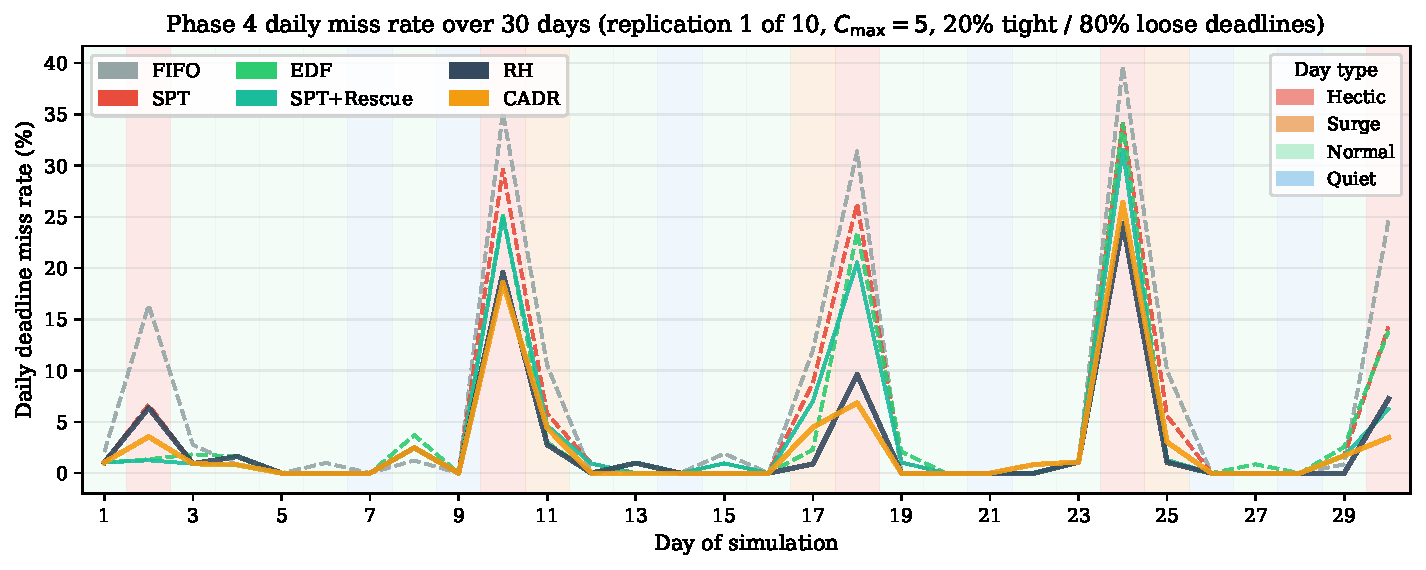
\includegraphics[width=0.98\linewidth,height=0.72\textheight,keepaspectratio]{figures/phase4_timeline.pdf}
\caption[Daily miss rate over the simulated month]{Daily deadline miss rate over 30 simulation days (replication~1 of 10, $C_{\max}=5$). Background shading indicates day type: red for hectic, orange for surge, green for normal, blue for quiet. RH (dark) and CADR (gold) are typically among the lowest spikes on hectic days, though EDF and SPT+Rescue occasionally match or beat them on individual days; FIFO (grey) provides the deadline-oblivious reference among the six policies shown. On normal and quiet days all schedulers converge near zero. The temporal structure confirms that scheduler choice is consequential only on the two heavy day types (hectic, above saturation, and surge, below saturation on execution load but with provisioning delays building a long queue), consistent with the Phase~3 day-type sensitivity analysis (Section~\ref{ssec:day-type-sensitivity-c-max-5}).}
\label{fig:phase4-timeline}
\end{figure}
\end{landscape}

On the continuous calendar RH and CADR are the two lowest-miss point estimates: RH \PhFourRHMiss\% and CADR \PhFourCADRMiss\%. RH records \PhFourRHWait~min wait and CADR \PhFourCADRwait~min, both above SPT (\PhFourSPTwait~min) and slightly below SPT+Rescue (\PhFourRescueWait~min). RH has the lower miss point estimate and CADR the lower tardiness (\PhFourCADRTard~min against \PhFourRHtard~min). No paired policy-comparison test is reported at Phase~4, so these differences describe point estimates rather than an established separation, and at $\times 1.25$ availability or under the data-ordered ranking CADR (among others) leads RH (Section~\ref{ssec:availability-model-sensitivity}). The Phase~3 paired evidence remains the basis for statements about statistical ties or superiority.

The reservation ablation measures a different question on the same ten monthly calendars and seeds. Disabling RH's anticipation lowers mean wait by \MonthResWaitDelta~min ($\MonthResWaitP$) while raising miss by \MonthResMissDelta~percentage points ($\MonthResMissP$) and mean tardiness by \MonthResTardDelta~min ($\MonthResTardP$). These are uncorrected paired tests, reported separately from the Phase~3 family. With anticipation off, RH records \MonthResOffWait~min wait and \MonthResOffMiss\% miss. The gate remains active on surge, normal and quiet days, is disabled on hectic days, and is also disabled while the final backlog drains after the calendar closes. Thus the monthly anticipation trade-off is measured under a persistent queue.

CADR's main advantage is miss severity: \PhFourCADRTard~min mean tardiness against RH's \PhFourRHtard~min. Figure~\ref{fig:tardiness_tradeoff} shows that neither proposed scheduler dominates the other on miss and tardiness: RH has the lower miss point estimate, CADR the lower tardiness. The Adaptive hybrid has the lowest monthly mean tardiness of all ten policies (\PhFourAdaptiveTard~min), below EDF's \PhFourEDFtard~min, but has higher miss (\PhFourAdaptiveMiss\%) than both proposed schedulers. CADR remains the recommended default for the combination of low miss and lower lateness, with RH preferred when the breach count is the overriding concern in the scarce baseline model; the small monthly miss difference is not presented as a tested advantage.

\begin{landscape}
\begin{figure}[H]
\centering
\captionsetup{font=small,skip=6pt}
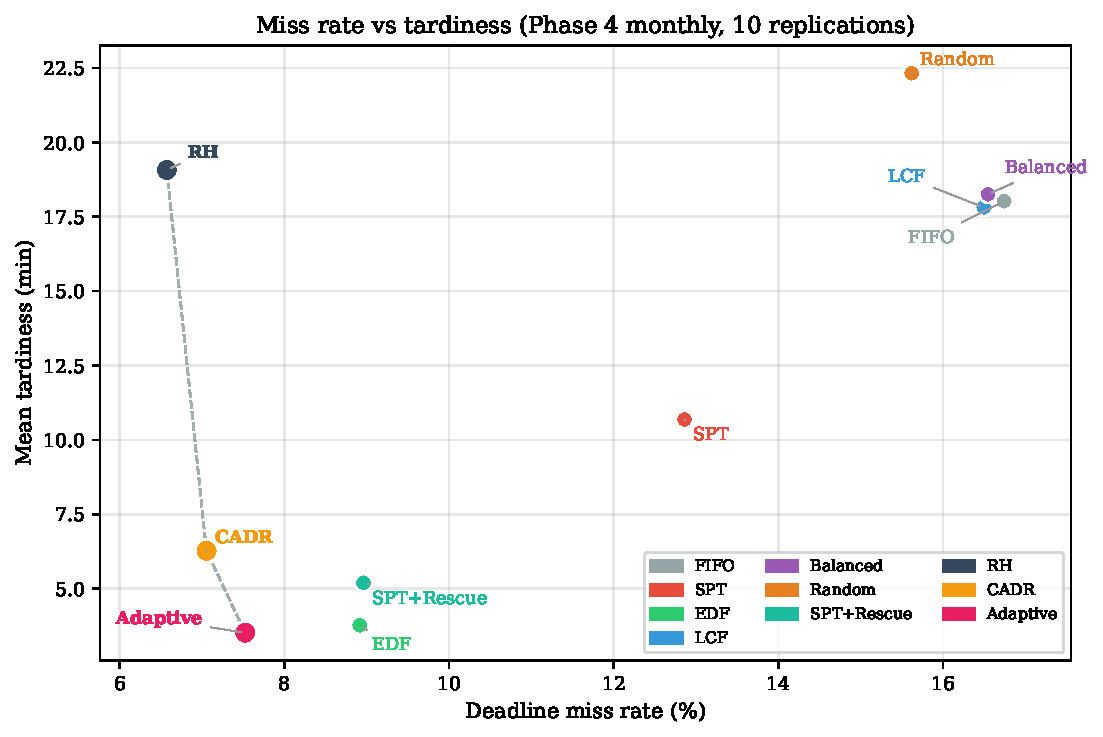
\includegraphics[width=0.98\linewidth,height=0.75\textheight,keepaspectratio]{figures/tardiness_tradeoff.pdf}
\caption[Miss rate vs tardiness trade-off]{Miss rate versus mean tardiness, continuous Phase~4 calendar ($C_{\max}=5$, ten replications). RH and CADR occupy the lowest-miss region (\PhFourRHMiss\% and \PhFourCADRMiss\%); RH has lower miss and CADR lower tardiness (\PhFourRHtard~min and \PhFourCADRTard~min). The Adaptive hybrid holds the lowest-tardiness end of the point-estimate frontier. No paired policy-comparison test is reported for this phase.}
\label{fig:tardiness_tradeoff}
\end{figure}
\end{landscape}

The Adaptive hybrid's \PhFourAdaptiveMiss\% miss improves on SPT+Rescue (\PhFourRescueMiss\%), EDF (\PhFourEDFmiss\%) and SPT (\PhFourSPTmiss\%), but RH and CADR both have lower miss and wait point estimates. EDF retains a low-tardiness profile, with \PhFourEDFmiss\% miss and \PhFourEDFwait~min wait; the Adaptive hybrid is numerically below it on miss and tardiness. Deadline-oblivious FIFO, LCF and Balanced remain substantially worse on miss, at \PhFourFIFOmiss\%, \PhFourLCFmiss\% and \PhFourBalancedMiss\% respectively. Both proposed schedulers reduce the FIFO monthly miss rate by more than half.

The hectic-day submission cohorts carry most of the missed deadlines: FIFO reaches \PhFourHecFIFOmiss\%, SPT \PhFourHecSPTmiss\%, and SPT+Rescue \PhFourHecRescueMiss\%. These cohort rates differ from the single-day Phase~3 estimates because the monthly experiment samples different job counts and seeds and retains queue and fleet state between days. The month is therefore a separate operational experiment, not a weighted average of independent daily benchmarks.

\section{Summary of Findings}
\label{sec:summary-of-findings}

Table~\ref{tab:findings} consolidates the key empirical findings from all phases.

\footnotesize
\begin{singlespace}
\begin{longtable}{>{\RaggedRight}p{0.29\textwidth} >{\RaggedRight}p{0.27\textwidth} >{\RaggedRight}p{0.33\textwidth}}
\caption{Summary of key experimental findings}\label{tab:findings}\\
\toprule
\textbf{Finding} & \textbf{Quantitative evidence} & \textbf{Practical implication} \\
\midrule
\endfirsthead
\toprule
\textbf{Finding} & \textbf{Quantitative evidence} & \textbf{Practical implication} \\
\midrule
\endhead
\bottomrule
\endfoot
SPT achieves the lowest baseline wait under capacity saturation ($\rho>1$), tied with RH; EDF achieves significantly lower miss (hectic, 20\%/80\% deadlines) & \SPTwait~min wait ($d=\SPTFIFOwaitD$ vs FIFO, $p<0.001$); \SPTmiss\% miss ($d=\SPTFIFOmissD$, $p<0.001$; EDF \EDFmiss\%, $p<0.001$), $n=30$ & SPT is the strongest low-wait baseline; the deadline-aware default is CADR, with RH the specialist for the scarce baseline regime (rows 1 and 4, Table~\ref{tab:rh_vs_cadr}) \\ \addlinespace
SPT+Rescue's laxity-rescue limits tight-deadline starvation under saturation & \RescueWait~min wait ($d=\RescueFIFOwaitD$, $p<0.001$); \RescueMiss\% miss ($d=\RescueFIFOmissD$, $p<0.001$) & Acceptable alternative when tight-deadline compliance is a strict requirement \\ \addlinespace
EDF achieves significantly lower miss than SPT; its wait is not significantly different from FIFO's & $d=\EDFFIFOmissD$ miss vs FIFO ($p<0.001$); $d=\EDFFIFOwaitD$ wait vs FIFO ($p=\EDFFIFOwaitP$, not significant) & EDF buys deadline safety with no wait advantage to show for it; prefer SPT when wait also matters \\ \addlinespace
Among the baseline policies in the sweep (surge, $\rho<1$), EDF's miss is significantly lower at $f_{\text{tight}} \leq 30\%$ and SPT's at $f_{\text{tight}} \geq 70\%$, their paired difference not significant at $f_{\text{tight}} = 50\%$ & EDF \DlTenEDFmiss\% vs SPT \DlTenSPTmiss\% at 10\% tight ($\DlTenSPTEDFmissP$); \DlFiftyEDFmiss\% vs \DlFiftySPTmiss\% at 50\% ($\DlFiftySPTEDFmissP$); SPT \DlSeventySPTmiss\% vs EDF \DlSeventyEDFmiss\% at 70\% ($\DlSeventySPTEDFmissP$) & Follow the tight-deadline-fraction boundary: EDF or SPT+Rescue for low tight fractions, SPT for high ones, either near the middle of the range \\ \addlinespace
RH achieves best-tier monthly miss (\PhFourRHMiss\%, near-identical to CADR); its monthly wait no longer leads, sitting within about two minutes of SPT's, CADR's and SPT+Rescue's & \PhFourRHMiss\% (RH) vs \PhFourFIFOmiss\% (FIFO); RH wait \PhFourRHWait~min vs SPT \PhFourSPTwait~min & At monthly scale RH and CADR have the two lowest miss point estimates (RH marginally lower, no paired test), consistent with CADR as the default; any preference for RH on miss count rests on Phase~3, and RH's wait advantage does not persist to monthly scale \\ \addlinespace
CADR achieves near-RH miss at substantially lower tardiness; matches SPT+Rescue's wait rather than beating it & Phase~3: \CADRmiss\% miss, \CADRtard~min tardiness vs RH \RHtard~min; Phase~4: \PhFourCADRMiss\% miss, \PhFourCADRTard~min tardiness vs RH \PhFourRHtard~min & Deploy CADR as the default: the Phase~3 miss difference from RH is not significant ($p=\RHCADRmissP$), but equivalence is untested; CADR has close monthly miss point estimates with lower tardiness, and leads under eased availability and the data-ordered ranking, and cuts tardiness substantially; keep RH for the scarce baseline regime when the lowest miss count is what matters (SPT where queue wait is the priority) \\ \addlinespace
\end{longtable}
\end{singlespace}
\normalsize

} % end \sloppy
